\documentclass{report}

%%%%%%%%%%%%%%%%%%%%%%%%%%%%%%%%%
% PACKAGE IMPORTS
%%%%%%%%%%%%%%%%%%%%%%%%%%%%%%%%%


\usepackage[tmargin=2cm,rmargin=1in,lmargin=1in,margin=0.85in,bmargin=2cm,footskip=.2in]{geometry}
\usepackage{amsmath,amsfonts,amsthm,amssymb,mathtools}
\usepackage[varbb]{newpxmath}
\usepackage{xfrac}
\usepackage[makeroom]{cancel}
\usepackage{mathtools}
\usepackage{bookmark}
\usepackage{enumitem}
\usepackage{hyperref,theoremref}
\hypersetup{
	pdftitle={Assignment},
	colorlinks=true, linkcolor=doc!90,
	bookmarksnumbered=true,
	bookmarksopen=true
}
\usepackage[most,many,breakable]{tcolorbox}
\usepackage{xcolor}
\usepackage{varwidth}
\usepackage{varwidth}
\usepackage{etoolbox}
%\usepackage{authblk}
\usepackage{nameref}
\usepackage{multicol,array}
\usepackage{tikz-cd}
\usepackage[ruled,vlined,linesnumbered]{algorithm2e}
\usepackage{comment} % enables the use of multi-line comments (\ifx \fi) 
\usepackage{import}
\usepackage{xifthen}
\usepackage{pdfpages}
\usepackage{transparent}

\newcommand\mycommfont[1]{\footnotesize\ttfamily\textcolor{blue}{#1}}
\SetCommentSty{mycommfont}
\newcommand{\incfig}[1]{%
    \def\svgwidth{\columnwidth}
    \import{./figures/}{#1.pdf_tex}
}

\usepackage{tikzsymbols}
\renewcommand\qedsymbol{$\Laughey$}


%\usepackage{import}
%\usepackage{xifthen}
%\usepackage{pdfpages}
%\usepackage{transparent}


%%%%%%%%%%%%%%%%%%%%%%%%%%%%%%
% SELF MADE COLORS
%%%%%%%%%%%%%%%%%%%%%%%%%%%%%%



\definecolor{myg}{RGB}{56, 140, 70}
\definecolor{myb}{RGB}{45, 111, 177}
\definecolor{myr}{RGB}{199, 68, 64}
\definecolor{mytheorembg}{HTML}{F2F2F9}
\definecolor{mytheoremfr}{HTML}{00007B}
\definecolor{mylenmabg}{HTML}{FFFAF8}
\definecolor{mylenmafr}{HTML}{983b0f}
\definecolor{mypropbg}{HTML}{f2fbfc}
\definecolor{mypropfr}{HTML}{191971}
\definecolor{myexamplebg}{HTML}{F2FBF8}
\definecolor{myexamplefr}{HTML}{88D6D1}
\definecolor{myexampleti}{HTML}{2A7F7F}
\definecolor{mydefinitbg}{HTML}{E5E5FF}
\definecolor{mydefinitfr}{HTML}{3F3FA3}
\definecolor{notesgreen}{RGB}{0,162,0}
\definecolor{myp}{RGB}{197, 92, 212}
\definecolor{mygr}{HTML}{2C3338}
\definecolor{myred}{RGB}{127,0,0}
\definecolor{myyellow}{RGB}{169,121,69}
\definecolor{myexercisebg}{HTML}{F2FBF8}
\definecolor{myexercisefg}{HTML}{88D6D1}


%%%%%%%%%%%%%%%%%%%%%%%%%%%%
% TCOLORBOX SETUPS
%%%%%%%%%%%%%%%%%%%%%%%%%%%%

\setlength{\parindent}{1cm}
%================================
% THEOREM BOX
%================================

\tcbuselibrary{theorems,skins,hooks}
\newtcbtheorem[number within=section]{Theorem}{Theorem}
{%
	enhanced,
	breakable,
	colback = mytheorembg,
	frame hidden,
	boxrule = 0sp,
	borderline west = {2pt}{0pt}{myg},
	sharp corners,
	detach title,
	before upper = \tcbtitle\par\smallskip,
	coltitle = myg,
	fonttitle = \bfseries\sffamily,
	description font = \mdseries,
	separator sign none,
	segmentation style={solid, mytheoremfr},
}
{th}

\tcbuselibrary{theorems,skins,hooks}
\newtcbtheorem[number within=chapter]{theorem}{Theorem}
{%
	enhanced,
	breakable,
	colback = mytheorembg,
	frame hidden,
	boxrule = 0sp,
	borderline west = {2pt}{0pt}{mytheoremfr},
	sharp corners,
	detach title,
	before upper = \tcbtitle\par\smallskip,
	coltitle = mytheoremfr,
	fonttitle = \bfseries\sffamily,
	description font = \mdseries,
	separator sign none,
	segmentation style={solid, mytheoremfr},
}
{th}


\tcbuselibrary{theorems,skins,hooks}
\newtcolorbox{Theoremcon}
{%
	enhanced
	,breakable
	,colback = mytheorembg
	,frame hidden
	,boxrule = 0sp
	,borderline west = {2pt}{0pt}{mytheoremfr}
	,sharp corners
	,description font = \mdseries
	,separator sign none
}

%================================
% Corollery
%================================
\tcbuselibrary{theorems,skins,hooks}
\newtcbtheorem[number within=section]{Corollary}{Corollary}
{%
	enhanced
	,breakable
	,colback = myp!10
	,frame hidden
	,boxrule = 0sp
	,borderline west = {2pt}{0pt}{myp!85!black}
	,sharp corners
	,detach title
	,before upper = \tcbtitle\par\smallskip
	,coltitle = myp!85!black
	,fonttitle = \bfseries\sffamily
	,description font = \mdseries
	,separator sign none
	,segmentation style={solid, myp!85!black}
}
{th}
\tcbuselibrary{theorems,skins,hooks}
\newtcbtheorem[number within=chapter]{corollary}{Corollary}
{%
	enhanced
	,breakable
	,colback = myp!10
	,frame hidden
	,boxrule = 0sp
	,borderline west = {2pt}{0pt}{myp!85!black}
	,sharp corners
	,detach title
	,before upper = \tcbtitle\par\smallskip
	,coltitle = myp!85!black
	,fonttitle = \bfseries\sffamily
	,description font = \mdseries
	,separator sign none
	,segmentation style={solid, myp!85!black}
}
{th}


%================================
% LENMA
%================================

\tcbuselibrary{theorems,skins,hooks}
\newtcbtheorem[number within=section]{Lenma}{Lenma}
{%
	enhanced,
	breakable,
	colback = mylenmabg,
	frame hidden,
	boxrule = 0sp,
	borderline west = {2pt}{0pt}{mylenmafr},
	sharp corners,
	detach title,
	before upper = \tcbtitle\par\smallskip,
	coltitle = mylenmafr,
	fonttitle = \bfseries\sffamily,
	description font = \mdseries,
	separator sign none,
	segmentation style={solid, mylenmafr},
}
{th}

\tcbuselibrary{theorems,skins,hooks}
\newtcbtheorem[number within=chapter]{lenma}{Lenma}
{%
	enhanced,
	breakable,
	colback = mylenmabg,
	frame hidden,
	boxrule = 0sp,
	borderline west = {2pt}{0pt}{mylenmafr},
	sharp corners,
	detach title,
	before upper = \tcbtitle\par\smallskip,
	coltitle = mylenmafr,
	fonttitle = \bfseries\sffamily,
	description font = \mdseries,
	separator sign none,
	segmentation style={solid, mylenmafr},
}
{th}


%================================
% PROPOSITION
%================================

\tcbuselibrary{theorems,skins,hooks}
\newtcbtheorem[number within=section]{Prop}{Proposition}
{%
	enhanced,
	breakable,
	colback = mypropbg,
	frame hidden,
	boxrule = 0sp,
	borderline west = {2pt}{0pt}{mypropfr},
	sharp corners,
	detach title,
	before upper = \tcbtitle\par\smallskip,
	coltitle = mypropfr,
	fonttitle = \bfseries\sffamily,
	description font = \mdseries,
	separator sign none,
	segmentation style={solid, mypropfr},
}
{th}

\tcbuselibrary{theorems,skins,hooks}
\newtcbtheorem[number within=chapter]{prop}{Proposition}
{%
	enhanced,
	breakable,
	colback = mypropbg,
	frame hidden,
	boxrule = 0sp,
	borderline west = {2pt}{0pt}{mypropfr},
	sharp corners,
	detach title,
	before upper = \tcbtitle\par\smallskip,
	coltitle = mypropfr,
	fonttitle = \bfseries\sffamily,
	description font = \mdseries,
	separator sign none,
	segmentation style={solid, mypropfr},
}
{th}


%================================
% CLAIM
%================================

\tcbuselibrary{theorems,skins,hooks}
\newtcbtheorem[number within=section]{claim}{Claim}
{%
	enhanced
	,breakable
	,colback = myg!10
	,frame hidden
	,boxrule = 0sp
	,borderline west = {2pt}{0pt}{myg}
	,sharp corners
	,detach title
	,before upper = \tcbtitle\par\smallskip
	,coltitle = myg!85!black
	,fonttitle = \bfseries\sffamily
	,description font = \mdseries
	,separator sign none
	,segmentation style={solid, myg!85!black}
}
{th}



%================================
% Exercise
%================================

\tcbuselibrary{theorems,skins,hooks}
\newtcbtheorem[number within=section]{Exercise}{Exercise}
{%
	enhanced,
	breakable,
	colback = myexercisebg,
	frame hidden,
	boxrule = 0sp,
	borderline west = {2pt}{0pt}{myexercisefg},
	sharp corners,
	detach title,
	before upper = \tcbtitle\par\smallskip,
	coltitle = myexercisefg,
	fonttitle = \bfseries\sffamily,
	description font = \mdseries,
	separator sign none,
	segmentation style={solid, myexercisefg},
}
{th}

\tcbuselibrary{theorems,skins,hooks}
\newtcbtheorem[number within=chapter]{exercise}{Exercise}
{%
	enhanced,
	breakable,
	colback = myexercisebg,
	frame hidden,
	boxrule = 0sp,
	borderline west = {2pt}{0pt}{myexercisefg},
	sharp corners,
	detach title,
	before upper = \tcbtitle\par\smallskip,
	coltitle = myexercisefg,
	fonttitle = \bfseries\sffamily,
	description font = \mdseries,
	separator sign none,
	segmentation style={solid, myexercisefg},
}
{th}

%================================
% EXAMPLE BOX
%================================

\newtcbtheorem[number within=section]{Example}{Example}
{%
	colback = myexamplebg
	,breakable
	,colframe = myexamplefr
	,coltitle = myexampleti
	,boxrule = 1pt
	,sharp corners
	,detach title
	,before upper=\tcbtitle\par\smallskip
	,fonttitle = \bfseries
	,description font = \mdseries
	,separator sign none
	,description delimiters parenthesis
}
{ex}

\newtcbtheorem[number within=chapter]{example}{Example}
{%
	colback = myexamplebg
	,breakable
	,colframe = myexamplefr
	,coltitle = myexampleti
	,boxrule = 1pt
	,sharp corners
	,detach title
	,before upper=\tcbtitle\par\smallskip
	,fonttitle = \bfseries
	,description font = \mdseries
	,separator sign none
	,description delimiters parenthesis
}
{ex}

%================================
% DEFINITION BOX
%================================

\newtcbtheorem[number within=section]{Definition}{Definition}{enhanced,
	before skip=2mm,after skip=2mm, colback=red!5,colframe=red!80!black,boxrule=0.5mm,
	attach boxed title to top left={xshift=1cm,yshift*=1mm-\tcboxedtitleheight}, varwidth boxed title*=-3cm,
	boxed title style={frame code={
					\path[fill=tcbcolback]
					([yshift=-1mm,xshift=-1mm]frame.north west)
					arc[start angle=0,end angle=180,radius=1mm]
					([yshift=-1mm,xshift=1mm]frame.north east)
					arc[start angle=180,end angle=0,radius=1mm];
					\path[left color=tcbcolback!60!black,right color=tcbcolback!60!black,
						middle color=tcbcolback!80!black]
					([xshift=-2mm]frame.north west) -- ([xshift=2mm]frame.north east)
					[rounded corners=1mm]-- ([xshift=1mm,yshift=-1mm]frame.north east)
					-- (frame.south east) -- (frame.south west)
					-- ([xshift=-1mm,yshift=-1mm]frame.north west)
					[sharp corners]-- cycle;
				},interior engine=empty,
		},
	fonttitle=\bfseries,
	title={#2},#1}{def}
\newtcbtheorem[number within=chapter]{definition}{Definition}{enhanced,
	before skip=2mm,after skip=2mm, colback=red!5,colframe=red!80!black,boxrule=0.5mm,
	attach boxed title to top left={xshift=1cm,yshift*=1mm-\tcboxedtitleheight}, varwidth boxed title*=-3cm,
	boxed title style={frame code={
					\path[fill=tcbcolback]
					([yshift=-1mm,xshift=-1mm]frame.north west)
					arc[start angle=0,end angle=180,radius=1mm]
					([yshift=-1mm,xshift=1mm]frame.north east)
					arc[start angle=180,end angle=0,radius=1mm];
					\path[left color=tcbcolback!60!black,right color=tcbcolback!60!black,
						middle color=tcbcolback!80!black]
					([xshift=-2mm]frame.north west) -- ([xshift=2mm]frame.north east)
					[rounded corners=1mm]-- ([xshift=1mm,yshift=-1mm]frame.north east)
					-- (frame.south east) -- (frame.south west)
					-- ([xshift=-1mm,yshift=-1mm]frame.north west)
					[sharp corners]-- cycle;
				},interior engine=empty,
		},
	fonttitle=\bfseries,
	title={#2},#1}{def}



%================================
% Solution BOX
%================================

\makeatletter
\newtcbtheorem{question}{Question}{
        enhanced,
	breakable,
	colback=white,
	colframe=myb!80!black,
	attach boxed title to top left={yshift*=-\tcboxedtitleheight},
	fonttitle=\bfseries,
	title={#2},
        boxed title size=title,
	boxed title style={%
			sharp corners,
			rounded corners=northwest,
			colback=tcbcolframe,
			boxrule=0pt,
		},
	underlay boxed title={%
			\path[fill=tcbcolframe] (title.south west)--(title.south east)
			to[out=0, in=180] ([xshift=5mm]title.east)--
			(title.center-|frame.east)
			[rounded corners=\kvtcb@arc] |-
			(frame.north) -| cycle;
		},
	#1
}{def}
\makeatother

%================================
% SOLUTION BOX
%================================

\makeatletter
\newtcolorbox{solution}{enhanced,
	breakable,
	colback=white,
	colframe=myg!80!black,
	attach boxed title to top left={yshift*=-\tcboxedtitleheight},
	title=Solution,
	boxed title size=title,
	boxed title style={%
			sharp corners,
			rounded corners=northwest,
			colback=tcbcolframe,
			boxrule=0pt,
		},
	underlay boxed title={%
			\path[fill=tcbcolframe] (title.south west)--(title.south east)
			to[out=0, in=180] ([xshift=5mm]title.east)--
			(title.center-|frame.east)
			[rounded corners=\kvtcb@arc] |-
			(frame.north) -| cycle;
		},
}
\makeatother

%================================
% Question BOX
%================================

\makeatletter
\newtcbtheorem{qstion}{Question}{enhanced,
	breakable,
	colback=white,
	colframe=mygr,
	attach boxed title to top left={yshift*=-\tcboxedtitleheight},
	fonttitle=\bfseries,
	title={},
	boxed title size=title,
	boxed title style={%
			sharp corners,
			rounded corners=northwest,
			colback=tcbcolframe,
			boxrule=0pt,
		},
	underlay boxed title={%
			\path[fill=tcbcolframe] (title.south west)--(title.south east)
			to[out=0, in=180] ([xshift=5mm]title.east)--
			(title.center-|frame.east)
			[rounded corners=\kvtcb@arc] |-
			(frame.north) -| cycle;
		},
	#1
}{def}
\makeatother

\newtcbtheorem[number within=chapter]{wconc}{Wrong Concept}{
	breakable,
	enhanced,
	colback=white,
	colframe=myr,
	arc=0pt,
	outer arc=0pt,
	fonttitle=\bfseries\sffamily\large,
	colbacktitle=myr,
	attach boxed title to top left={},
	boxed title style={
			enhanced,
			skin=enhancedfirst jigsaw,
			arc=3pt,
			bottom=0pt,
			interior style={fill=myr}
		},
	#1
}{def}



%================================
% NOTE BOX
%================================

\usetikzlibrary{arrows,calc,shadows.blur}
\tcbuselibrary{skins}
\newtcolorbox{note}[1][]{%
	enhanced jigsaw,
	colback=gray!20!white,%
	colframe=gray!80!black,
	size=small,
	boxrule=1pt,
	title=\textbf{Note:-},
	halign title=flush center,
	coltitle=black,
	breakable,
	drop shadow=black!50!white,
	attach boxed title to top left={xshift=1cm,yshift=-\tcboxedtitleheight/2,yshifttext=-\tcboxedtitleheight/2},
	minipage boxed title=1.5cm,
	boxed title style={%
			colback=white,
			size=fbox,
			boxrule=1pt,
			boxsep=2pt,
			underlay={%
					\coordinate (dotA) at ($(interior.west) + (-0.5pt,0)$);
					\coordinate (dotB) at ($(interior.east) + (0.5pt,0)$);
					\begin{scope}
						\clip (interior.north west) rectangle ([xshift=3ex]interior.east);
						\filldraw [white, blur shadow={shadow opacity=60, shadow yshift=-.75ex}, rounded corners=2pt] (interior.north west) rectangle (interior.south east);
					\end{scope}
					\begin{scope}[gray!80!black]
						\fill (dotA) circle (2pt);
						\fill (dotB) circle (2pt);
					\end{scope}
				},
		},
	#1,
}

\newtcolorbox{exercice}[1][]{%
	enhanced jigsaw,
	colback=gray!20!white,%
	colframe=gray!80!black,
	size=small,
	boxrule=1pt,
	title=\textbf{Exercice},
	halign title=flush center,
	coltitle=black,
	breakable,
	drop shadow=black!50!white,
	attach boxed title to top left={xshift=1cm,yshift=-\tcboxedtitleheight/2,yshifttext=-\tcboxedtitleheight/2},
	minipage boxed title=1.5cm,
	boxed title style={%
			colback=white,
			size=fbox,
			boxrule=1pt,
			boxsep=2pt,
			underlay={%
					\coordinate (dotA) at ($(interior.west) + (-0.5pt,0)$);
					\coordinate (dotB) at ($(interior.east) + (0.5pt,0)$);
					\begin{scope}
						\clip (interior.north west) rectangle ([xshift=3ex]interior.east);
						\filldraw [white, blur shadow={shadow opacity=60, shadow yshift=-.75ex}, rounded corners=2pt] (interior.north west) rectangle (interior.south east);
					\end{scope}
					\begin{scope}[gray!80!black]
						\fill (dotA) circle (2pt);
						\fill (dotB) circle (2pt);
					\end{scope}
				},
		},
	#1,
}

%%%%%%%%%%%%%%%%%%%%%%%%%%%%%%
% SELF MADE COMMANDS
%%%%%%%%%%%%%%%%%%%%%%%%%%%%%%


\newcommand{\thm}[2]{\begin{Theorem}{#1}{}#2\end{Theorem}}
\newcommand{\cor}[2]{\begin{Corollary}{#1}{}#2\end{Corollary}}
\newcommand{\mlenma}[2]{\begin{Lenma}{#1}{}#2\end{Lenma}}
\newcommand{\mprop}[2]{\begin{Prop}{#1}{}#2\end{Prop}}
\newcommand{\clm}[3]{\begin{claim}{#1}{#2}#3\end{claim}}
\newcommand{\wc}[2]{\begin{wconc}{#1}{}\setlength{\parindent}{1cm}#2\end{wconc}}
\newcommand{\thmcon}[1]{\begin{Theoremcon}{#1}\end{Theoremcon}}
\newcommand{\ex}[2]{\begin{Example}{#1}{}#2\end{Example}}
\newcommand{\dfn}[2]{\begin{Definition}[colbacktitle=red!75!black]{#1}{}#2\end{Definition}}
\newcommand{\dfnc}[2]{\begin{definition}[colbacktitle=red!75!black]{#1}{}#2\end{definition}}
\newcommand{\qs}[2]{\begin{question}{#1}{}#2\end{question}}
\newcommand{\pf}[2]{\begin{myproof}[#1]#2\end{myproof}}
\newcommand{\nt}[1]{\begin{note}#1\end{note}}
\newcommand{\exr}[1]{\begin{exercice}#1\end{exercice}}

\newcommand*\circled[1]{\tikz[baseline=(char.base)]{
		\node[shape=circle,draw,inner sep=1pt] (char) {#1};}}
\newcommand\getcurrentref[1]{%
	\ifnumequal{\value{#1}}{0}
	{??}
	{\the\value{#1}}%
}
\newcommand{\getCurrentSectionNumber}{\getcurrentref{section}}
\newenvironment{myproof}[1][\proofname]{%
	\proof[\bfseries #1: ]%
}{\endproof}

\newcommand{\mclm}[2]{\begin{myclaim}[#1]#2\end{myclaim}}
\newenvironment{myclaim}[1][\claimname]{\proof[\bfseries #1: ]}{}

\newcounter{mylabelcounter}

\makeatletter
\newcommand{\setword}[2]{%
	\phantomsection
	#1\def\@currentlabel{\unexpanded{#1}}\label{#2}%
}
\makeatother




\tikzset{
	symbol/.style={
			draw=none,
			every to/.append style={
					edge node={node [sloped, allow upside down, auto=false]{$#1$}}}
		}
}


% deliminators
\DeclarePairedDelimiter{\abs}{\lvert}{\rvert}
\DeclarePairedDelimiter{\norm}{\lVert}{\rVert}

\DeclarePairedDelimiter{\ceil}{\lceil}{\rceil}
\DeclarePairedDelimiter{\floor}{\lfloor}{\rfloor}
\DeclarePairedDelimiter{\round}{\lfloor}{\rceil}

\newsavebox\diffdbox
\newcommand{\slantedromand}{{\mathpalette\makesl{d}}}
\newcommand{\makesl}[2]{%
\begingroup
\sbox{\diffdbox}{$\mathsurround=0pt#1\mathrm{#2}$}%
\pdfsave
\pdfsetmatrix{1 0 0.2 1}%
\rlap{\usebox{\diffdbox}}%
\pdfrestore
\hskip\wd\diffdbox
\endgroup
}
\newcommand{\dd}[1][]{\ensuremath{\mathop{}\!\ifstrempty{#1}{%
\slantedromand\@ifnextchar^{\hspace{0.2ex}}{\hspace{0.1ex}}}%
{\slantedromand\hspace{0.2ex}^{#1}}}}
\ProvideDocumentCommand\dv{o m g}{%
  \ensuremath{%
    \IfValueTF{#3}{%
      \IfNoValueTF{#1}{%
        \frac{\dd #2}{\dd #3}%
      }{%
        \frac{\dd^{#1} #2}{\dd #3^{#1}}%
      }%
    }{%
      \IfNoValueTF{#1}{%
        \frac{\dd}{\dd #2}%
      }{%
        \frac{\dd^{#1}}{\dd #2^{#1}}%
      }%
    }%
  }%
}
\providecommand*{\pdv}[3][]{\frac{\partial^{#1}#2}{\partial#3^{#1}}}
%  - others
\DeclareMathOperator{\Lap}{\mathcal{L}}
\DeclareMathOperator{\Var}{Var} % varience
\DeclareMathOperator{\Cov}{Cov} % covarience
\DeclareMathOperator{\E}{E} % expected

% Since the amsthm package isn't loaded

% I prefer the slanted \leq
\let\oldleq\leq % save them in case they're every wanted
\let\oldgeq\geq
\renewcommand{\leq}{\leqslant}
\renewcommand{\geq}{\geqslant}

% % redefine matrix env to allow for alignment, use r as default
% \renewcommand*\env@matrix[1][r]{\hskip -\arraycolsep
%     \let\@ifnextchar\new@ifnextchar
%     \array{*\c@MaxMatrixCols #1}}


%\usepackage{framed}
%\usepackage{titletoc}
%\usepackage{etoolbox}
%\usepackage{lmodern}


%\patchcmd{\tableofcontents}{\contentsname}{\sffamily\contentsname}{}{}

%\renewenvironment{leftbar}
%{\def\FrameCommand{\hspace{6em}%
%		{\color{myyellow}\vrule width 2pt depth 6pt}\hspace{1em}}%
%	\MakeFramed{\parshape 1 0cm \dimexpr\textwidth-6em\relax\FrameRestore}\vskip2pt%
%}
%{\endMakeFramed}

%\titlecontents{chapter}
%[0em]{\vspace*{2\baselineskip}}
%{\parbox{4.5em}{%
%		\hfill\Huge\sffamily\bfseries\color{myred}\thecontentspage}%
%	\vspace*{-2.3\baselineskip}\leftbar\textsc{\small\chaptername~\thecontentslabel}\\\sffamily}
%{}{\endleftbar}
%\titlecontents{section}
%[8.4em]
%{\sffamily\contentslabel{3em}}{}{}
%{\hspace{0.5em}\nobreak\itshape\color{myred}\contentspage}
%\titlecontents{subsection}
%[8.4em]
%{\sffamily\contentslabel{3em}}{}{}  
%{\hspace{0.5em}\nobreak\itshape\color{myred}\contentspage}



%%%%%%%%%%%%%%%%%%%%%%%%%%%%%%%%%%%%%%%%%%%
% TABLE OF CONTENTS
%%%%%%%%%%%%%%%%%%%%%%%%%%%%%%%%%%%%%%%%%%%

\usepackage{tikz}
\definecolor{doc}{RGB}{0,60,110}
\usepackage{titletoc}
\contentsmargin{0cm}
\titlecontents{chapter}[3.7pc]
{\addvspace{30pt}%
	\begin{tikzpicture}[remember picture, overlay]%
		\draw[fill=doc!60,draw=doc!60] (-7,-.1) rectangle (-0.9,.5);%
		\pgftext[left,x=-3.5cm,y=0.2cm]{\color{white}\Large\sc\bfseries Chapter\ \thecontentslabel};%
	\end{tikzpicture}\color{doc!60}\large\sc\bfseries}%
{}
{}
{\;\titlerule\;\large\sc\bfseries Page \thecontentspage
	\begin{tikzpicture}[remember picture, overlay]
		\draw[fill=doc!60,draw=doc!60] (2pt,0) rectangle (4,0.1pt);
	\end{tikzpicture}}%
\titlecontents{section}[3.7pc]
{\addvspace{2pt}}
{\contentslabel[\thecontentslabel]{2pc}}
{}
{\hfill\small \thecontentspage}
[]
\titlecontents*{subsection}[3.7pc]
{\addvspace{-1pt}\small}
{}
{}
{\ --- \small\thecontentspage}
[ \textbullet\ ][]

\makeatletter
\renewcommand{\tableofcontents}{%
	\chapter*{%
	  \vspace*{-20\p@}%
	  \begin{tikzpicture}[remember picture, overlay]%
		  \pgftext[right,x=15cm,y=0.2cm]{\color{doc!60}\Huge\sc\bfseries \contentsname};%
		  \draw[fill=doc!60,draw=doc!60] (13,-.75) rectangle (20,1);%
		  \clip (13,-.75) rectangle (20,1);
		  \pgftext[right,x=15cm,y=0.2cm]{\color{white}\Huge\sc\bfseries \contentsname};%
	  \end{tikzpicture}}%
	\@starttoc{toc}}
\makeatother


%From M275 "Topology" at SJSU
\newcommand{\id}{\mathrm{id}}
\newcommand{\taking}[1]{\xrightarrow{#1}}
\newcommand{\inv}{^{-1}}

%From M170 "Introduction to Graph Theory" at SJSU
\DeclareMathOperator{\diam}{diam}
\DeclareMathOperator{\ord}{ord}
\newcommand{\defeq}{\overset{\mathrm{def}}{=}}

%From the USAMO .tex files
\newcommand{\ts}{\textsuperscript}
\newcommand{\dg}{^\circ}
\newcommand{\ii}{\item}

% % From Math 55 and Math 145 at Harvard
% \newenvironment{subproof}[1][Proof]{%
% \begin{proof}[#1] \renewcommand{\qedsymbol}{$\blacksquare$}}%
% {\end{proof}}

\newcommand{\HRule}{\rule{\linewidth}{0.5mm}}
\newcommand{\liff}{\leftrightarrow}
\newcommand{\lthen}{\rightarrow}
\newcommand{\opname}{\operatorname}
\newcommand{\surjto}{\twoheadrightarrow}
\newcommand{\injto}{\hookrightarrow}
\newcommand{\On}{\mathrm{On}} % ordinals
\DeclareMathOperator{\img}{im} % Image
\DeclareMathOperator{\Img}{Im} % Image
\DeclareMathOperator{\coker}{coker} % Cokernel
\DeclareMathOperator{\Coker}{Coker} % Cokernel
\DeclareMathOperator{\Ker}{Ker} % Kernel
\DeclareMathOperator{\rank}{rank}
\DeclareMathOperator{\Spec}{Spec} % spectrum
\DeclareMathOperator{\Tr}{Tr} % trace
\DeclareMathOperator{\pr}{pr} % projection
\DeclareMathOperator{\ext}{ext} % extension
\DeclareMathOperator{\pred}{pred} % predecessor
\DeclareMathOperator{\dom}{dom} % domain
\DeclareMathOperator{\ran}{ran} % range
\DeclareMathOperator{\Hom}{Hom} % homomorphism
\DeclareMathOperator{\Mor}{Mor} % morphisms
\DeclareMathOperator{\End}{End} % endomorphism

\newcommand{\eps}{\epsilon}
\newcommand{\veps}{\varepsilon}
\newcommand{\ol}{\overline}
\newcommand{\ul}{\underline}
\newcommand{\wt}{\widetilde}
\newcommand{\wh}{\widehat}
\newcommand{\vocab}[1]{\textbf{\color{blue} #1}}
\providecommand{\half}{\frac{1}{2}}
\newcommand{\dang}{\measuredangle} %% Directed angle
\newcommand{\ray}[1]{\overrightarrow{#1}}
\newcommand{\seg}[1]{\overline{#1}}
\newcommand{\arc}[1]{\wideparen{#1}}
\DeclareMathOperator{\cis}{cis}
\DeclareMathOperator*{\lcm}{lcm}
\DeclareMathOperator*{\argmin}{arg min}
\DeclareMathOperator*{\argmax}{arg max}
\newcommand{\cycsum}{\sum_{\mathrm{cyc}}}
\newcommand{\symsum}{\sum_{\mathrm{sym}}}
\newcommand{\cycprod}{\prod_{\mathrm{cyc}}}
\newcommand{\symprod}{\prod_{\mathrm{sym}}}
\newcommand{\Qed}{\begin{flushright}\qed\end{flushright}}
\newcommand{\parinn}{\setlength{\parindent}{1cm}}
\newcommand{\parinf}{\setlength{\parindent}{0cm}}
% \newcommand{\norm}{\|\cdot\|}
\newcommand{\inorm}{\norm_{\infty}}
\newcommand{\opensets}{\{V_{\alpha}\}_{\alpha\in I}}
\newcommand{\oset}{V_{\alpha}}
\newcommand{\opset}[1]{V_{\alpha_{#1}}}
\newcommand{\lub}{\text{lub}}
\newcommand{\del}[2]{\frac{\partial #1}{\partial #2}}
\newcommand{\Del}[3]{\frac{\partial^{#1} #2}{\partial^{#1} #3}}
\newcommand{\deld}[2]{\dfrac{\partial #1}{\partial #2}}
\newcommand{\Deld}[3]{\dfrac{\partial^{#1} #2}{\partial^{#1} #3}}
\newcommand{\lm}{\lambda}
\newcommand{\uin}{\mathbin{\rotatebox[origin=c]{90}{$\in$}}}
\newcommand{\usubset}{\mathbin{\rotatebox[origin=c]{90}{$\subset$}}}
\newcommand{\lt}{\left}
\newcommand{\rt}{\right}
\newcommand{\bs}[1]{\boldsymbol{#1}}
\newcommand{\exs}{\exists}
\newcommand{\st}{\strut}
\newcommand{\dps}[1]{\displaystyle{#1}}

\newcommand{\sol}{\setlength{\parindent}{0cm}\textbf{\textit{Solution:}}\setlength{\parindent}{1cm} }
\newcommand{\solve}[1]{\setlength{\parindent}{0cm}\textbf{\textit{Solution: }}\setlength{\parindent}{1cm}#1 \Qed}

% Things Lie
\newcommand{\kb}{\mathfrak b}
\newcommand{\kg}{\mathfrak g}
\newcommand{\kh}{\mathfrak h}
\newcommand{\kn}{\mathfrak n}
\newcommand{\ku}{\mathfrak u}
\newcommand{\kz}{\mathfrak z}
\DeclareMathOperator{\Ext}{Ext} % Ext functor
\DeclareMathOperator{\Tor}{Tor} % Tor functor
\newcommand{\gl}{\opname{\mathfrak{gl}}} % frak gl group
\renewcommand{\sl}{\opname{\mathfrak{sl}}} % frak sl group chktex 6

% More script letters etc.
\newcommand{\SA}{\mathcal A}
\newcommand{\SB}{\mathcal B}
\newcommand{\SC}{\mathcal C}
\newcommand{\SF}{\mathcal F}
\newcommand{\SG}{\mathcal G}
\newcommand{\SH}{\mathcal H}
\newcommand{\OO}{\mathcal O}

\newcommand{\SCA}{\mathscr A}
\newcommand{\SCB}{\mathscr B}
\newcommand{\SCC}{\mathscr C}
\newcommand{\SCD}{\mathscr D}
\newcommand{\SCE}{\mathscr E}
\newcommand{\SCF}{\mathscr F}
\newcommand{\SCG}{\mathscr G}
\newcommand{\SCH}{\mathscr H}

% Mathfrak primes
\newcommand{\km}{\mathfrak m}
\newcommand{\kp}{\mathfrak p}
\newcommand{\kq}{\mathfrak q}

% number sets
\newcommand{\RR}[1][]{\ensuremath{\ifstrempty{#1}{\mathbb{R}}{\mathbb{R}^{#1}}}}
\newcommand{\NN}[1][]{\ensuremath{\ifstrempty{#1}{\mathbb{N}}{\mathbb{N}^{#1}}}}
\newcommand{\ZZ}[1][]{\ensuremath{\ifstrempty{#1}{\mathbb{Z}}{\mathbb{Z}^{#1}}}}
\newcommand{\QQ}[1][]{\ensuremath{\ifstrempty{#1}{\mathbb{Q}}{\mathbb{Q}^{#1}}}}
\newcommand{\CC}[1][]{\ensuremath{\ifstrempty{#1}{\mathbb{C}}{\mathbb{C}^{#1}}}}
\newcommand{\PP}[1][]{\ensuremath{\ifstrempty{#1}{\mathbb{P}}{\mathbb{P}^{#1}}}}
\newcommand{\HH}[1][]{\ensuremath{\ifstrempty{#1}{\mathbb{H}}{\mathbb{H}^{#1}}}}
\newcommand{\FF}[1][]{\ensuremath{\ifstrempty{#1}{\mathbb{F}}{\mathbb{F}^{#1}}}}
% expected value
\newcommand{\EE}{\ensuremath{\mathbb{E}}}
\newcommand{\charin}{\text{ char }}
\DeclareMathOperator{\sign}{sign}
\DeclareMathOperator{\Aut}{Aut}
\DeclareMathOperator{\Inn}{Inn}
\DeclareMathOperator{\Syl}{Syl}
\DeclareMathOperator{\Gal}{Gal}
\DeclareMathOperator{\GL}{GL} % General linear group
\DeclareMathOperator{\SL}{SL} % Special linear group

%---------------------------------------
% BlackBoard Math Fonts :-
%---------------------------------------

%Captital Letters
\newcommand{\bbA}{\mathbb{A}}	\newcommand{\bbB}{\mathbb{B}}
\newcommand{\bbC}{\mathbb{C}}	\newcommand{\bbD}{\mathbb{D}}
\newcommand{\bbE}{\mathbb{E}}	\newcommand{\bbF}{\mathbb{F}}
\newcommand{\bbG}{\mathbb{G}}	\newcommand{\bbH}{\mathbb{H}}
\newcommand{\bbI}{\mathbb{I}}	\newcommand{\bbJ}{\mathbb{J}}
\newcommand{\bbK}{\mathbb{K}}	\newcommand{\bbL}{\mathbb{L}}
\newcommand{\bbM}{\mathbb{M}}	\newcommand{\bbN}{\mathbb{N}}
\newcommand{\bbO}{\mathbb{O}}	\newcommand{\bbP}{\mathbb{P}}
\newcommand{\bbQ}{\mathbb{Q}}	\newcommand{\bbR}{\mathbb{R}}
\newcommand{\bbS}{\mathbb{S}}	\newcommand{\bbT}{\mathbb{T}}
\newcommand{\bbU}{\mathbb{U}}	\newcommand{\bbV}{\mathbb{V}}
\newcommand{\bbW}{\mathbb{W}}	\newcommand{\bbX}{\mathbb{X}}
\newcommand{\bbY}{\mathbb{Y}}	\newcommand{\bbZ}{\mathbb{Z}}

%---------------------------------------
% MathCal Fonts :-
%---------------------------------------

%Captital Letters
\newcommand{\mcA}{\mathcal{A}}	\newcommand{\mcB}{\mathcal{B}}
\newcommand{\mcC}{\mathcal{C}}	\newcommand{\mcD}{\mathcal{D}}
\newcommand{\mcE}{\mathcal{E}}	\newcommand{\mcF}{\mathcal{F}}
\newcommand{\mcG}{\mathcal{G}}	\newcommand{\mcH}{\mathcal{H}}
\newcommand{\mcI}{\mathcal{I}}	\newcommand{\mcJ}{\mathcal{J}}
\newcommand{\mcK}{\mathcal{K}}	\newcommand{\mcL}{\mathcal{L}}
\newcommand{\mcM}{\mathcal{M}}	\newcommand{\mcN}{\mathcal{N}}
\newcommand{\mcO}{\mathcal{O}}	\newcommand{\mcP}{\mathcal{P}}
\newcommand{\mcQ}{\mathcal{Q}}	\newcommand{\mcR}{\mathcal{R}}
\newcommand{\mcS}{\mathcal{S}}	\newcommand{\mcT}{\mathcal{T}}
\newcommand{\mcU}{\mathcal{U}}	\newcommand{\mcV}{\mathcal{V}}
\newcommand{\mcW}{\mathcal{W}}	\newcommand{\mcX}{\mathcal{X}}
\newcommand{\mcY}{\mathcal{Y}}	\newcommand{\mcZ}{\mathcal{Z}}


%---------------------------------------
% Bold Math Fonts :-
%---------------------------------------

%Captital Letters
\newcommand{\bmA}{\boldsymbol{A}}	\newcommand{\bmB}{\boldsymbol{B}}
\newcommand{\bmC}{\boldsymbol{C}}	\newcommand{\bmD}{\boldsymbol{D}}
\newcommand{\bmE}{\boldsymbol{E}}	\newcommand{\bmF}{\boldsymbol{F}}
\newcommand{\bmG}{\boldsymbol{G}}	\newcommand{\bmH}{\boldsymbol{H}}
\newcommand{\bmI}{\boldsymbol{I}}	\newcommand{\bmJ}{\boldsymbol{J}}
\newcommand{\bmK}{\boldsymbol{K}}	\newcommand{\bmL}{\boldsymbol{L}}
\newcommand{\bmM}{\boldsymbol{M}}	\newcommand{\bmN}{\boldsymbol{N}}
\newcommand{\bmO}{\boldsymbol{O}}	\newcommand{\bmP}{\boldsymbol{P}}
\newcommand{\bmQ}{\boldsymbol{Q}}	\newcommand{\bmR}{\boldsymbol{R}}
\newcommand{\bmS}{\boldsymbol{S}}	\newcommand{\bmT}{\boldsymbol{T}}
\newcommand{\bmU}{\boldsymbol{U}}	\newcommand{\bmV}{\boldsymbol{V}}
\newcommand{\bmW}{\boldsymbol{W}}	\newcommand{\bmX}{\boldsymbol{X}}
\newcommand{\bmY}{\boldsymbol{Y}}	\newcommand{\bmZ}{\boldsymbol{Z}}
%Small Letters
\newcommand{\bma}{\boldsymbol{a}}	\newcommand{\bmb}{\boldsymbol{b}}
\newcommand{\bmc}{\boldsymbol{c}}	\newcommand{\bmd}{\boldsymbol{d}}
\newcommand{\bme}{\boldsymbol{e}}	\newcommand{\bmf}{\boldsymbol{f}}
\newcommand{\bmg}{\boldsymbol{g}}	\newcommand{\bmh}{\boldsymbol{h}}
\newcommand{\bmi}{\boldsymbol{i}}	\newcommand{\bmj}{\boldsymbol{j}}
\newcommand{\bmk}{\boldsymbol{k}}	\newcommand{\bml}{\boldsymbol{l}}
\newcommand{\bmm}{\boldsymbol{m}}	\newcommand{\bmn}{\boldsymbol{n}}
\newcommand{\bmo}{\boldsymbol{o}}	\newcommand{\bmp}{\boldsymbol{p}}
\newcommand{\bmq}{\boldsymbol{q}}	\newcommand{\bmr}{\boldsymbol{r}}
\newcommand{\bms}{\boldsymbol{s}}	\newcommand{\bmt}{\boldsymbol{t}}
\newcommand{\bmu}{\boldsymbol{u}}	\newcommand{\bmv}{\boldsymbol{v}}
\newcommand{\bmw}{\boldsymbol{w}}	\newcommand{\bmx}{\boldsymbol{x}}
\newcommand{\bmy}{\boldsymbol{y}}	\newcommand{\bmz}{\boldsymbol{z}}

%---------------------------------------
% Scr Math Fonts :-
%---------------------------------------

\newcommand{\sA}{{\mathscr{A}}}   \newcommand{\sB}{{\mathscr{B}}}
\newcommand{\sC}{{\mathscr{C}}}   \newcommand{\sD}{{\mathscr{D}}}
\newcommand{\sE}{{\mathscr{E}}}   \newcommand{\sF}{{\mathscr{F}}}
\newcommand{\sG}{{\mathscr{G}}}   \newcommand{\sH}{{\mathscr{H}}}
\newcommand{\sI}{{\mathscr{I}}}   \newcommand{\sJ}{{\mathscr{J}}}
\newcommand{\sK}{{\mathscr{K}}}   \newcommand{\sL}{{\mathscr{L}}}
\newcommand{\sM}{{\mathscr{M}}}   \newcommand{\sN}{{\mathscr{N}}}
\newcommand{\sO}{{\mathscr{O}}}   \newcommand{\sP}{{\mathscr{P}}}
\newcommand{\sQ}{{\mathscr{Q}}}   \newcommand{\sR}{{\mathscr{R}}}
\newcommand{\sS}{{\mathscr{S}}}   \newcommand{\sT}{{\mathscr{T}}}
\newcommand{\sU}{{\mathscr{U}}}   \newcommand{\sV}{{\mathscr{V}}}
\newcommand{\sW}{{\mathscr{W}}}   \newcommand{\sX}{{\mathscr{X}}}
\newcommand{\sY}{{\mathscr{Y}}}   \newcommand{\sZ}{{\mathscr{Z}}}


%---------------------------------------
% Math Fraktur Font
%---------------------------------------

%Captital Letters
\newcommand{\mfA}{\mathfrak{A}}	\newcommand{\mfB}{\mathfrak{B}}
\newcommand{\mfC}{\mathfrak{C}}	\newcommand{\mfD}{\mathfrak{D}}
\newcommand{\mfE}{\mathfrak{E}}	\newcommand{\mfF}{\mathfrak{F}}
\newcommand{\mfG}{\mathfrak{G}}	\newcommand{\mfH}{\mathfrak{H}}
\newcommand{\mfI}{\mathfrak{I}}	\newcommand{\mfJ}{\mathfrak{J}}
\newcommand{\mfK}{\mathfrak{K}}	\newcommand{\mfL}{\mathfrak{L}}
\newcommand{\mfM}{\mathfrak{M}}	\newcommand{\mfN}{\mathfrak{N}}
\newcommand{\mfO}{\mathfrak{O}}	\newcommand{\mfP}{\mathfrak{P}}
\newcommand{\mfQ}{\mathfrak{Q}}	\newcommand{\mfR}{\mathfrak{R}}
\newcommand{\mfS}{\mathfrak{S}}	\newcommand{\mfT}{\mathfrak{T}}
\newcommand{\mfU}{\mathfrak{U}}	\newcommand{\mfV}{\mathfrak{V}}
\newcommand{\mfW}{\mathfrak{W}}	\newcommand{\mfX}{\mathfrak{X}}
\newcommand{\mfY}{\mathfrak{Y}}	\newcommand{\mfZ}{\mathfrak{Z}}
%Small Letters
\newcommand{\mfa}{\mathfrak{a}}	\newcommand{\mfb}{\mathfrak{b}}
\newcommand{\mfc}{\mathfrak{c}}	\newcommand{\mfd}{\mathfrak{d}}
\newcommand{\mfe}{\mathfrak{e}}	\newcommand{\mff}{\mathfrak{f}}
\newcommand{\mfg}{\mathfrak{g}}	\newcommand{\mfh}{\mathfrak{h}}
\newcommand{\mfi}{\mathfrak{i}}	\newcommand{\mfj}{\mathfrak{j}}
\newcommand{\mfk}{\mathfrak{k}}	\newcommand{\mfl}{\mathfrak{l}}
\newcommand{\mfm}{\mathfrak{m}}	\newcommand{\mfn}{\mathfrak{n}}
\newcommand{\mfo}{\mathfrak{o}}	\newcommand{\mfp}{\mathfrak{p}}
\newcommand{\mfq}{\mathfrak{q}}	\newcommand{\mfr}{\mathfrak{r}}
\newcommand{\mfs}{\mathfrak{s}}	\newcommand{\mft}{\mathfrak{t}}
\newcommand{\mfu}{\mathfrak{u}}	\newcommand{\mfv}{\mathfrak{v}}
\newcommand{\mfw}{\mathfrak{w}}	\newcommand{\mfx}{\mathfrak{x}}
\newcommand{\mfy}{\mathfrak{y}}	\newcommand{\mfz}{\mathfrak{z}}


\graphicspath{{./img}}

\title{\Huge{Théorie du transport optimal}}
\author{\huge{Racine Florian}}


\renewcommand{\contentsname}{Table des matières}
\renewcommand{\listfigurename}{Liste des figures}

\begin{document}

\maketitle
\newpage
\pdfbookmark[section]{\contentsname}{toc}
\tableofcontents
\pagebreak

\chapter{Cours}
\section{Introduction}
\subsection{Formulation du problème}
\qs{}{Quelle est la façon optimal de transporter un tas de sable dans un trou ?}
\qs{}{Comment constuire un chateau de sable d'une forme données à partir d'un tas de sable ?}

\begin{figure}[htpb]
    \centering
    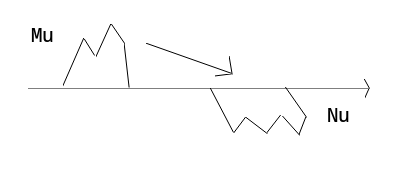
\includegraphics[width=0.8\textwidth]{intro}
    \caption{Transporter un tas de sable dans un trou}
\end{figure}

\nt{ Avec le même nombre de grain de sable et la même masse.}

\section{Modélisation}
$\nu \in \mathcal{P}(\mathbb{R})$ ; $\mu \in \mathcal{P}(\mathbb{R})$
\dfn{}{$\forall A \in \mathcal{P} (\mathbb{R}),\mu[A]$ décrit quelle quantité de sable est dans A.
}
\begin{figure}[htpb]
    \centering
    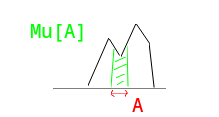
\includegraphics[width=0.3\textwidth]{partieMu}
    \caption{$\mu[A]$}
\end{figure}

\dfn{}{
Cout infinitésimal :
\begin{displaymath}
C:
\left|
  \begin{array}{rcl}
      \mathbb{R}*\mathbb{R} & \longrightarrow & \mathbb{R} \\
      (x,y) & \longmapsto & C(x,y) \\
  \end{array}
\right.
\end{displaymath}
Cout de transporter un grain de sable de x vers y.
}
\qs{}{Comment transporter un tas de sable avec un cout global minimal ?}
\dfn{}{
Un plan de transport entre les mesures $\mu$  et  $\nu$ est une mesure de probabilité : \\
$\Pi \in \mathcal{P}(\mathbb{R}*\mathbb{R})$ à pour marginale $\mu$ et $\nu$.
}

\nt{
$\Pi \in \mathcal{P}(\mathbb{R}*\mathbb{R})$ à pour marginal $\mu$ et $\nu$ \\
$\Leftrightarrow \forall $A,B enssemble mesurable avec A$ \subset \mathbb{R}$ et B $\subset \mathbb{R}$
$\left\{
\begin{array}{l}
\Pi[A\times\mathbb{R}] = \mu[A] \\
\Pi[\mathbb{R}\times B] = \mu[B]
\end{array}
\right.$\\
$\Leftrightarrow \forall \varphi \in C^{0}(\mathbb{R}), \Psi \in C^{0}(\mathbb{R}) : $
$\displaystyle \int_{{\mathbb{R} \times \mathbb{R}}} {\varphi (x) + \Psi (y)} \: d{\Pi (x,y)}$
$= \displaystyle \int {\varphi (x)} \: d{\mu (x)}$
}

\nt{
On notera, $\Pi ( \mu , \nu )$ = \{ $\Pi \in \mathcal{P} (\mathbb{R} \times \mathbb{R}) | \Pi$
a pour marginal, $\mu, \nu$ \}\\
On remarquera que, $\Pi ( \mu , \nu ) \neq \varnothing $\\
$I[\Pi] = \displaystyle \int_{\mathbb{R}^{2}} {C(x,y)} \: d{\Pi (x,y)}$ Le cout total assocé au plan de transport optimal.\\

On cherche, $\tau_{c} (\mu , \nu ) = INF_{\Pi \in \Pi(\mu, \nu)} (I[\Pi])$
}

\dfn{}{
    S'il existe $\Pi_{0} \in \mathcal{P} ( \mathbb{R} \times \mathbb{R} )$
    tel que $I[\Pi_{0}] = \tau_{c} (\mu , \nu)$\\
    $\Pi_{0}$ est appelé un \bf{plan de transfert optimal}
}


\ex{Exemple trivial (Kotorovitch)}{
$a < b$\\
$c < d$\\
$C(x,y) = |x-y|^{2}$\\
$\mu = \frac{1}{2} (\delta_{a} + \delta_{b})$\\
$\nu = \frac{1}{2} (\delta_{c} + \delta_{d})$
\qs{}{
$\Pi ( \mu , \nu) = ?$
}
\sol{
$\Pi_{\alpha} = \frac{1}{2} ( \alpha \delta_{(a,c)} + (1 - \alpha ) \delta_{(a,d)} + (1 - \alpha ) \delta_{(b,c)} + \alpha \delta_{(b,d)})$
\boldmath
$\Pi(\mu,\nu) = \{\Pi_{\alpha} | \alpha \in [0, 1] \}$
\unboldmath
}
\qs{}{
    Calculer : $I[ \Pi ] \forall \Pi \in \Pi( \mu , \nu )$
}
\sol{
    $I[\Pi_{\alpha}] = \displaystyle \int_{\mathbb{R}^{2}} {C(x,y)} \: d{\Pi_{\alpha} (x,y)}$\\
    $I[\Pi_{\alpha}] = \frac{1}{2}(\alpha C(a,c) + (1 - \alpha) C(a,d) + (1 - \alpha) C(b,c) + \alpha C(b,d)) $\\
    $I[\Pi_{\alpha}] = \frac{1}{2}(a^{2}+b^{2}+c^{2}+d^{2}) - \alpha (ac + bd) -(1 - \alpha) (ad+ cb)$
}
\qs{}{
    Trouver : $\tau_{c}( \mu , \nu )$
}
\sol{
$P(\alpha) =  \frac{\partial I[\Pi_{\alpha}]}{\partial \alpha}$
$\implies P(\alpha) = -ac - bd + ad + cb$;
$\implies P(\alpha) = (d-c)(a-b) < 0$\\
Donc, $I[\Pi_{\alpha}]$ atteint son min en $\alpha = 1$\\
$\Pi_{0} = \Pi_{\alpha = 1}$\\
Donc, $a \rightarrow c$ et, $b \rightarrow d$
}
}
\begin{figure}[htpb]
   \centering
    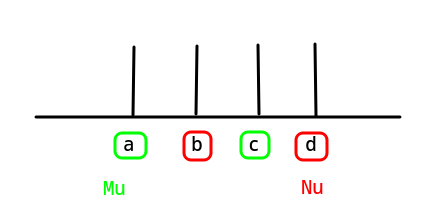
\includegraphics[width=0.4\textwidth]{exemple1}
    \caption{Solution}
\end{figure}
\section{La formulation du problème de transfert optimal de Monge}
\nt{
On autorise pas le fait de couper les masses.
A chaque x est associé une unique y.\\
On dit que T envoie $\mu$ sur $\nu$ et on note : $T \# \mu = \nu$
}
\mprop{}{
    $\forall A \subset \mathbb{R}$ partie mesurable : $\nu(A) = \mu(T^{-1}(A))$
}
$\Leftrightarrow$
\mprop{}{
    $\forall \varphi$ continue :$\displaystyle\int_{\mathbb{R}} {\varphi (y)} \: d{\nu (y)} = $
    $\displaystyle \int_{\mathbb{R}} {(\varphi o T)(x)} \: d{\mu (x)}$\\
    $\tau_{c}^{M} (\mu , \nu) = INF_{T tq T \#f = \nu} I[T]$\\
    $I(T) = \displaystyle\int_{\mathbb{R}} {C(x,T(x))} \: d{\mu (x)}$
}
\nt{
Solution de cout optimal d'après Kantorovitch $\le$ Solution de cout optimal d'après Monge\\
Dans le première exemple ils coincident.\\
}
\nt{
Kantorovitch définit un problème linéare en $\Pi$.\\
Monge définit un problème non linéare en T.
}

\nt{
    Problème de kantorovitch admet toujours une solution $\Pi_{0}$.\\
    Problème de Monge n'admet pas toujours de solution n'y même d'application qui envoi $\mu$ sur $\nu$.
}
\ex{}{
$\left\{
\begin{array}{l}
\mu \in \mathcal{P}(\mathbb{R})\\
\nu = \delta_{a}\\
\end{array}
\right.$\\
    \textbf{Kantorovitch :} $\Pi(\mu , \nu) = \{ \mu \otimes \delta_{a} \}$\\
    \textbf{Monge :} Quelles sont les T tel que $T\# \mu = \nu$ ?\\
    Il en existe une seule: 
    \begin{displaymath}
    \forall x | T:
    \left|
      \begin{array}{rcl}
        x & \longrightarrow & a \\
        \mathbb{R} & \longmapsto & \mathbb{R} \\
      \end{array}
    \right.
    \end{displaymath}
    $\tau_{c}^{M} (\mu , \nu) = \tau_{c} (\mu , \nu)$\\
    D'une part : \\
    $\tau_{c}^{M} (\mu , \nu) = \displaystyle\int_{\mathbb{R}} {C(T(x),x)} \: d{\mu (x)}$\\
    $\tau_{c}^{M} (\mu , \nu) = \displaystyle\int_{\mathbb{R}} {C(0,x)} \: d{\mu (x)}$\\
    D'autre part : \\
    $\tau_{c} (\mu , \nu) = \displaystyle\int_{\mathbb{R}} {C(x,y)} \: d{\Pi (x,y)}$\\
    $\tau_{c} (\mu , \nu) = \displaystyle\int_{\mathbb{R}} {C(x,y)} \: d{(\mu \otimes \delta_{a})(x,y)}$\\
    $\tau_{c} (\mu , \nu) = \displaystyle\int_{\mathbb{R}} {C(x,y)} \: d{\mu (x)} d{\delta_{a}}$\\
    $\tau_{c} (\mu , \nu) = \displaystyle\int_{\mathbb{R}} {C(x,0)} \: d{\mu (x)}$\\
}

\ex{}{
$\left\{
\begin{array}{l}
    \mu = \frac{1}{n} \sum_{i=1}^{n} \delta_{x_{i}}\\
    \nu = \frac{1}{n} \sum_{i=1}^{n} \delta_{y_{i}}\\
\end{array}
\right.$\\
Les plans de transports $\Pi$ entre $\mu$ et $\nu$ peuvent être représenté par des matrices bistochastiques de tailles n.\\
$0 \le \Pi_{i,j} \le 1$\\
$\sum_{i=1}^{n} \Pi_{i,j} = 1$\\
$\sum_{j=1}^{n} \Pi_{i,j} = 1$\\
\nt{
On note $\mathcal{B}_{n}$ l'enssemble des matrices bisctochastiques.\\
}
Soit $\Pi \in \mathcal{B}_{n}$ : $I[\Pi] = \frac{1}{n} \sum_{i=1}^{n} C(x_{i}, y_{i}) \Pi_{i,j}$\\
$\tau_{c}(\mu ,\nu) = INF_{\Pi \in \mathcal{B}_{n}} \{\frac{1}{n}\sum_{i=1}^{n} \Pi_{i,j} C(x_{i}, y_{i})$\\
    Il s'agit d'un problème linéaire de minimisation sur un enssemble convexe.\\
}
\mprop{Enssemble convexe}{
    $\mathcal{B}_{n}$ est convexe $\Leftrightarrow A,B \in \mathcal{B}_{n}$ alors $\forall \theta \in [0,1] | \theta A + (1 - \theta ) B \in \mathcal{B}_{n}$
}
\dfn{Points extremaux}
{
    L'enssemble des points extremaux de E convexe est l'enssemble des $e \in E$ tel que :\\
    si $e=\theta e_{1} + (1 - \theta ) e_{2}$ avec $\theta \in [0, 1], e_{1} \in E, e_{2} \in E$\\
    Alors $\theta = 0$ ou $\theta = 1$
}
\thm{Théorème de Choquet}{
F est linéaire sur un domaine K convexe et compact, alors F admet au moin un minimum.
Parmi les minimums de F au moin l'un d'eux est un extrema de K.
}
\thm{Théorème de Birkhoff}{
    $\mathcal{B}_{n}$ est convexe et compact.\\
$\mathcal{B}_{n}$ admet n points extremaux qui sont les matrices de permutations\\
Ainsi, le min pour le problème de Kantorovitch est atteint pour
$\left\{
\begin{array}{l}
    \Pi_{i,j} = 1 | si j = \sigma(i)\\
    \Pi_{i,j} = 0 | sinon\\
\end{array}
\right.$\\
}

\section{La dualité de Kantorovitch}
\subsection{La théorie}%

\thm{Dualité de Kantorovitch}{
    $\mu \in \mathcal{P} (\mathbb{R}^{n}) ;$ $\nu \in \mathcal{P} (\mathbb{R}^{n})$\\
    C semi continue inférieurement ( par exemple C continue)
    \nt{ Pour $\Pi \in \Pi(\mu , \nu), I[\Pi] = \displaystyle \int_{{}}^{{}} {C(x,y)} \: d{\Pi(x,y)}$ }
    Soit $(\varphi, \psi ) \in \phi_{c}$\\
    $J(\varphi, \psi) = \displaystyle \int_{\mathbb{R}^{n}} {\varphi(x)} \: d{\mu (x)}$
    $+ \displaystyle \int_{\mathbb{R}^{n}} {\psi(y)} \: d{\nu (y)}$\\
    $\phi_{c} = \{ (\varphi, \psi) \in (\mathcal{C}^{0}( \mathbb{R}^{n} ))^{2}$ tq $\varphi (x) + \psi(y) \le C(x,y)$ presque partout $\}$\\
    Alors, $INF_{\Pi \in \Pi(\mu, \nu)}I[\Pi] = SUP_{(\varphi , \psi) \in \phi_{c}} J(\varphi , \psi)$
}
\nt{
    Interprétation :\\
    \begin{enumerate}
        \item On embauche un transporteur.\\
        \item Il achète de la masse située en x au pris $\varphi(x)$.\\
        \item Il vous débarasse au prix $\displaystyle \int {\varphi(x)} \: d{\mu(x)}$\\
        \item Il vous revend de la masse en y au prix $\psi(y)$\\
        \item On rachète $\nu$ au prix $\displaystyle \int {\psi(y)} \: d{\nu(y)}$\\
    \end{enumerate}
    On embauche le transporteur sous la condition : $\varphi(x) + \psi(y) \leq C(x,y)$
}
\begin{myproof}
    D'une part : \\
    Soit $(\varphi , \psi ) \in \phi_{c}$\\
    Soit $\Pi \in \Pi(\mu, \nu) | I[\Pi] ) \tau(\mu , \nu)$

    $J(\varphi, \psi) = \displaystyle \int_{\mathbb{R}^{n}} {\varphi(x)} \: d{\mu (x)}$
    $+ \displaystyle \int_{\mathbb{R}^{n}} {\psi(y)} \: d{\nu (y)}$
    $\le \displaystyle \int {C(x,y)} \: d{\Pi(x,y)}$
    $= I[\Pi] = \tau(\mu,\nu) = INF_{\Pi} I[\Pi]$\\
    Ainsi, $J(\varphi , \psi) \le INF_{\Pi} I[Pi]$
    
    D'autre part :\\
    
    
\end{myproof}

\dfn{Les fonction C-concaves (relatif au coût)}{
    Soit, $\varphi : \mathbb{R}^{n} \rightarrow \mathbb{R} \cup \{-\infty\}$\\
    On définit sa fonction C-conjuguée par :
    \begin{displaymath}
    \varphi^{c}:
    \left|
      \begin{array}{rcl}
          \mathbb{R}^{n} \ & \longrightarrow & \mathbb{R} \cup - \{\infty\} \\
          y & \longmapsto & INF_{x \in \mathbb{R}^{n}} (C(x,y) - \varphi(x)) \\
      \end{array}
    \right.
    \end{displaymath}
    On dit que $\varphi$ est C-concave si $\exists \psi : \mathbb{R}^{n} \rightarrow \mathbb{R} \cup \{- \infty \}$ tq
    $\forall x \in \mathbb{R}^{n}, \varphi (x) = \psi^{c}(x)$
}

\mlenma{}{
    \begin{enumerate}
        \item $\forall(x,y) \in \mathbb{R}^{n} \times \mathbb{R}^{n}, \varphi(x) + \varphi^{c}(y) \le C(x,y)$
        \item $\varphi^{c} = \varphi^{ccc} $
        \item $\varphi = \varphi^{cc} \Leftrightarrow \varphi $ est C-concave
    \end{enumerate}
}
\begin{myproof}
    \begin{enumerate}
        \item 
            Par définition, $\forall y, \varphi^{c}(y) = INF_{x \in \mathbb{R}^{n}} (C(x,y) - \varphi(x)) \le C(x,y) - \varphi(x) \forall x \in \mathbb{R}^{n}$\\
            Ainsi, $\forall(x,y) \in \mathbb{R}^{n} \times \mathbb{R}^{n}, \varphi(x) + \varphi^{c}(y) \le C(x,y)$\\

        \item 
            Par définition, $\varphi^{cc}(y) = INF_{x \in \mathbb{R}^{n}} (C(x,y) - \varphi^{c}(x)) \ge \varphi(y)$\\
            En effet comme démontré ci-dessus, $\forall (x,y)\in \mathbb{R}^{n} \times \mathbb{R}^{n},\varphi(y) \le C(x,y) - \varphi^{c}(x)$\\

            $\Rightarrow$
            D'une part, $\varphi^{c}(x) = INF_{y} (C(x,y) - \varphi(y))$
            $\ge INF_{y} (C(x,y) - \varphi^{cc}(y)) = \varphi^{ccc}(x)$\\
            \boldmath
            Ainsi, $\varphi^{c}(x) \ge \varphi^{ccc}(x)$
            \unboldmath

            $\Rightarrow$
            Et d'autre part, $INF_{x \in \mathbb{R}^{n}} (C(x,y) - \varphi^{c}(x)) \le C(x,y) - \varphi^{c}(x) \forall (x,y)\in \mathbb{R}^{n} \times \mathbb{R}^{n}$\\
            Donc, $\forall (x,y)\in \mathbb{R}^{n} \times \mathbb{R}^{n}, \varphi^{c}(x) \le C(x,y) - \varphi^{cc}(x)$\\
            Donc, $\forall (x,y)\in \mathbb{R}^{n} \times \mathbb{R}^{n}, \varphi^{c}(x) \le INF_{x \in \mathbb{R}^{n}} (C(x,y) - \varphi^{cc}(x))$
            $ = \varphi^{ccc}(x))$\\
            \boldmath
            Ainsi, $\varphi^{c}(x) \le \varphi^{ccc}(x))$\\
            \unboldmath

            \boldmath
            Ce qui montre bien que,$\varphi^{c}(x) = \varphi^{ccc}(x)$
            \unboldmath

        \item
            $\Rightarrow$
            Si $\varphi$ est C-concave alors $\exists \psi | \varphi = \psi^{c}$\\
            Donc, $\varphi^{cc} = \psi^{ccc} = \psi^{c} = \varphi$\\
            $\Leftarrow$
            Si $\varphi = \varphi^{cc}, alors \varphi = (\varphi^{c})^{c}$ Donc $\varphi$ est C-concave.
    \end{enumerate}
\end{myproof}

\thm{}{
    La dualité de Kantorovitch peut être restreinte à des couples de fonction C-conjuguées.\\
    $SUP_{(\varphi , \psi) \in (C(\mathbb{R}^{n})^{2}} J(\varphi, \psi) = MAX_{(\psi^{c} , \psi)} J(\psi^{c} , \psi)$
}

\begin{myproof}
    On montre que le sup est un max.
\end{myproof}

\cor{Les plans de transferts optimals sont caractérisés par leur support}{
    Si $(\varphi , \psi)$ est un maximiseur pour le problème de Kantorovitch dual, alors\\
    $\Pi \in \Pi(\mu , \nu)$ est un minimiseur pour le problème de Kantorovitch primal si et seulement si $\Pi$ est concentrée sur
    $\{ (x,y) \in \mathbb{R}^{n} \times \mathbb{R}^{n} | \varphi (x) + \psi(y) = C(x,y) \}$
}

\subsection{Application(s)}
\mprop{
On considère un objet indexé par j présent en quantité $\nu_{j}$.\\
(type(j), quantjté(j)) = (j, $\nu_{j}$)\\
On considère un consomateur indexé par i présent en quantité $\mu_{i}$.\\
(type(i), quantité(i)) = (i, $\mu_{i}$)\\
Utilité de l'objet j pour l'agent i.\\
\textbf{Hypothèse} L'utilité est tranférable.\\
L'objet j a une utilité nette $U_{r,j} - P$.\\
Pour un système de prix $P_{j}$, l'agent i choisit l'objet $j_{p}$ qui maximise  $U_{ij} - P_{j}$.\\
Transfert optimal: $SUP_{\Pi} \sum_{ij} U_{ij} \Pi_{ij}$ sous la contrainte $\sum_{j}  \Pi_{ij} = \mu_{i}$ $; \sum_{i}  \Pi_{ij} = \nu_{j}$ 
}

\nt{
    \textbf{Explication :}\\
    $\mu = \sum_{i} \mu_{i} \delta_{x_{i}}$\\
    $\nu = \sum_{j} \nu_{j} \delta_{y_{j}}$\\
    $C(i,j) = - u_{i,j}$\\
    $I[\Pi] = - \sum_{ij} u_{ij} \Pi_{ij}$\\
    \textbf{Utilité maximale :} $INF_{\Pi} I[\Pi] = SUP_{\Pi} \{ - \sum_{i} \varphi_{i} \mu_{i} - \sum_{j} \psi_{j} \nu{j} \}$\\
    \textbf{Problème dual :} $(D) : INF_{P_{j}} \{ \sum_{j} \nu_{j} P_{j} + \sum_{i} \mu_{i} MAX_{j} (\nu{ij} - P{j}) \}$
}

\dfn{Prix d'équilibre}{
    Un système de prix qui satisfait (D) est un prix d'équilibre du problème.
    Un tel système de prix permet d'atteindre l'optimum global
}

\nt{
    Pour le mar. 29 nov. 2022\\
    Lire Guillaume Carlier, Teaching, Transfert Optimal (Chapitre 3 Matching equilibre)\\
    Faire exercice 5, 6, 8 et 9.
}

\section{La distance de Wasserstein}

\dfn{Distance de Wasserstein}{
    On munit $\mathbb{R}^{n}$ d'une distance d.
    On considère la fonction cout : $C(x,y) = [d(x,y)]^{p}$
    Par convention, si $p = 0$, par convention, $(d(x,y))^{0} =$
    $\left\{
    \begin{array}{l}
         = 0 | si x=y\\
        = 1 | sinon\\
    \end{array}
    \right.$\\
}

\dfn{}{
    $\mathcal{P}_{p}(\mathbb{R}^{n})$
}

\nt{
    Si $p \in \mathcal{P}_{p}(\mathbb{R}^{n})$ alors $\forall y \in \mathbb{R}^{n}$,
    $\displaystyle \int {d(y,x)^{p}} \: d{\mu(x)} < \infty$\\
    Si d est borné $\mathcal{P}_{p}(\mathbb{R}^{n}) = \mathcal{P}(\mathbb{R}^{n})$ 
}

\dfn{}{
    Soit $p \ge 1$\\
    On définit, $W^{p}_{p}(\mu, \nu) = INF_{\pi \in \Pi (\mu, \nu)} \int_{\mathbb{R}^n \times \mathbb{R}^n} {d(x,y)^{p}} \: d{\pi(x,y)}$\\
    \nt{
        On remarque que,
        $W_{p}(\mu, \nu) = [\tau_{p}(\mu,\nu)]^{\frac{1}{p}}$
    }
}

\mlenma{Lemme de }{
}

\thm{}{
    $W^{p}$ est une mesure

}

\begin{myproof}
.
\dfn{Inégalité Triangulaire}{
    Soient $\mu_{1}, \mu_{2}, \mu_{3} \in \mathcal{P}_{p}(\mathbb{R}^{n})$
    $\pi_{1,2}(\mu_{1}) = \mu_{2}$
    $\pi_{2,3}(\mu_{2}) = \mu_{3}$\\
    Des plans de transports optimaux.
    On note $\pi$ la mesure de proba sur $\mathbb{R}^{n} \times \mathbb{R}^{n} \times \mathbb{R}^{n}$ définie dans le lemme définit ci-dessous.\\
    On note $\pi_{1,3}$ sa marginale sur $\mathbb{R}^{n} \times \mathbb{R}^{n}$ \\
    On a $\pi_{1,3} \in \Pi(\mu_{1}, \mu_{3})$ mais pas ( forcément ) optimal.
    \nt{
        $\Pi$ à pour marginale $\pi_{1,3}$ sur $\mathbb{R}_{1}^{n} \times \mathbb{R}_{2}^{n}$\\
        $\forall \varphi \in \mathcal(\mathbb{R}^{n} \times \mathbb{R}^{n})$
        $\int {\varphi(x,y)} \: d{\Pi(x,y,z)}$
        $= \int {\varphi(x,y)} \: d{\pi_{1,3}(x,y)}$
        
    }
}
\end{myproof}

\ex{}{
    $p=2$ \\
   $W_{2}$ est la distance de Wasserstein quadratique.\\
    Si $\mu \in \mathcal{P}_{2}(\mathbb{R}^{n}), a \in \mathbb{R}^{n}$\\
    $W_2 (\mu, \delta_a ) = \int_{\mathbb{R}^n} {(x-a)^{2}} \: d{\mu (x)}$\\
    Et la moyenne de $\mu$ (son esperance) est définie comme : $m = \int {x d\mu(x)} \: d{x}$\\
    $m = INF_{a \in \mathbb{R}^{n}} W_2 (\mu , \delta_a)$\\
    \nt{
        Cela permet de définir des espérances sur des espaces compliqués dans lesquels on ne peut pas définir d'intégrale.
    }
}

\ex{}{
$p=1$\\
$\tau_1$ s'appelle la distance de Rubinstein-Kantorovitch.
}

\mprop{}{

}

\ex{}{
    Le cas $\mathbb{R}^{n} = \mathbb{R}$
}

\dfn{CDF}{
    $\mu \in \mathcal{P}(\mathbb{R})$
    On définit sa CDF par :
    $F(x) = \int {} \: d{} {}$
    
}

\dfn{}{
    On appelle $F^{-1}$ l'inverse généralisé de F définie sur [0,1] par :
    $F^{-1} (t) = INF_{x \in \mathbb{R} | F(x) > t}$
}

\mprop{}{
    $W_{1}(\mu, \nu) = \int_{{0}}^{{1}} {F^{-1} (t) - G^{-1}(t)} \: d{t}$\\
    $W_{1}(\mu, \nu) = \int_{\mathbb{R}} {|F (x) - G(x)|} \: d{x}$\\
    $W_{1}(\mu, \nu) = ||F - G||_{L_1(\mathbb{R})}$
}

\nt{
    On note, $\mu_1, \ldots, \mu_n \in \mathcal{P}_{2}(\mathbb{R}^{n})$\\
$\lambda_1, \ldots, \lambda_n \in \mathbb{R}^{+}$
tel que $\sum_{i=1}^{n} \lambda_i = 1$
}

\dfn{}{
    $\mu^{*} = INF_{\mu \in \mathcal{P}_2 (\mathbb{R})} \sum_{i=1}^{n} \lambda_i W_{2}^{2} (\mu , \mu_i)$\\
    est le barycentre de $(\mu_1, \nu_1) \ldots (\mu_n, \lambda_n)$
}

\nt{
    Voir cours :
    Peyré / Cuturi : Computational Transfert optimal.
}

\section{Estimation numérique du transfert optimal}
\subsection{L'algorithme de Sinkhorn}

\nt{
Permet de calculer le transfert optimal entre 2 mesures
}

\subsubsection{Le contexte}
\nt {
    Habituellement présenté dans le cas discret (cela permet de facilement implémenter l'algorithme numériquement)\\
    $a = \sum_{i=1}^{n} a_i \delta_{x_{i}}$
    $b = \sum_{j=1}^{m} b_j \delta_{y_{j}}$ \\
    $C_{ij} = C(x_i,y_j)$ C correspond à une fonction cout\\
    $ \tau (a,b) = INF\{ \sum_{i,j} C_{ij} P_{ij} | P \in M_{n * m} (\mathcal{R}) \}$ P est une mesure de probabilité \\
    $P \mathbb{1}_{n} = a$
    et 
    $tp \mathbb{1}_n = b$
    Avec , $\mathbb{1}_m = (1, 1, 1, \ldots , 1)$ m fois
}

\subsubsection{Régulation entropique}
\paragraph{Formulation}
.
\dfn{L'entropie de couplage}{
    L'entropique discrète d'une matrice de couplage (une matrice qui envoi une mesure a sur une mesure b)\\
    $H(P) = \sum_{i,j} P_{ij} ((log P_{ij}) - 1)$\\
    Avec, P une matrice bistochastique (la somme des éléments de chaque colonne vaut 1)
}

\nt{
    Remarque  le terme -1 ne sert à rien.\\
    On pourrait avoir :
    $H(P) = \sum_{i,j} P_{ij} ((log P_{ij}))$\\
    car,\\
    $\sum_{i,j} P_{ij} = 1$\\
    $\int d\pi = 1 $ avec $\pi \in \mathcal{P} (\mathbb{R}^{n} \times \mathbb{R}^{n})$
}
\mprop{}{
    $H: M_{n \times m}(\mathbb{R}) \rightarrow \mathbb{R}^{+}$\\

    $\nabla H(P) = (log(P_{ij}) + 1)_{i,j}$\\
    $\nabla^{2} H(P) = diag(\frac{1}{P_{ij}})$\\
    $diag(P_{ij})$ Correspond a une matrice avec tous les termes de P sur la diagonale
}
\begin{myproof}
    Montrons que, $\nabla H(P) = (log(P_{ij})_{i,j}$\\
    $(P, Q) \in (M_{n \times m} (\mathbb{R}))^{2}$\\
    $H(P+ \delta Q) = H(P) + \delta < \nabla H(P) , Q > + \frac{\delta ^{2}}{2} <\nabla^{2} H(P) Q, Q> + \theta (\delta^{2})$
    Formule Taylor\\
    $H(P + \delta Q) = \sum_{ij} ((P_{ij} + \delta Q_{ij}) log(P_{ij} + \delta Q_{ij})$
    Par définition \\
    En developpant la formule de la définition on montre qu'elle est égale à la formule de Taylor
    On la développe à l'aide d'un développement limité sur le log.
\end{myproof}

\nt{
    Tout cela permet de montrer que l'entropie est \textbf{convexe} sur l'ensemble des matrices bistochastiques (qui est un ensemble convexe)
}

\exr{
Parmi les couplage P, quels sont ceux qui minimisent l'entropie ?\\
}

\sol{
    Soit $P^*$ un min de H sous la contrainte $\sum_{ij} P_{ij} = 1$\\
    Avec, $F(P^*) = 0$ ou $F(P) = \sum_{ij} P_{ij} - 1$
    Ce qui correspond à un problème d'optimisation sous contrainte.\\
    Alors, $\exists \lambda \in \mathbb{R}$ tq $\nabla H (P^{*}) + \lambda \nabla F(P^{*}) = 0$
    et, $F(P^{*}) = 0$\\
    $\forall ij (log P_{ij} + 1 + \lambda) = 0$\\
    $\forall ij  P_{ij} = \frac{1}{nm}$\\

    Donc l'entropie est minimal lorsque tous les points de a sont coupler avec tous les points de b.
}

\exr{
    $\tau^{\varepsilon} = INF_{P \in \Pi(a,b)} \{ <P, C> + \varepsilon H(P)\}$\\
    C'est un problème d'optimisation (comme pour le probleme de transfert optimal) mais la fonction à minimiser est convexe.
    En effet c'est la somme d'une fonction convexe et d'une fonction linéaire. 
    Minimiser une fonction convexe est beaucoup plus simple que de minimiser une fonction linéaire.\\
    On notera se problème : 
    $(T.O^{\varepsilon})$
}

\thm{}{
    La solution $(P^{\varepsilon})$ de $(T.O^{\varepsilon})$\\
    \begin{itemize}
        \item   
    converge vers le couplage d'entropie minimal : $a \otimes b = a^{t}b$ quand $\varepsilon \rightarrow \mathcal{1}$
        \item
    converge vers $P^{0}$ quand $\varepsilon \rightarrow 0$\\
            Ou $P^{0} = argmax\{H(P)\}$
    \end{itemize}
    $P \in \Pi(a,b)$
    $<P,C> = \tau^{c}(a,b)$
}

\begin{myproof}
    On note $(P^{\varepsilon})$ l'unique solution de $(T.O^{\varepsilon})$\\
    $\forall \varepsilon P^{\varepsilon} \in \Pi(a,b)$ qui est borné\\
    On peut extraire une sous suite $P^{\varepsilon} \rightarrow P^{0}$\\
    $\Pi(a,b)$ est fermé dans $M_{n\times m}(\mathbb{R})$\\
    Donc, $P^{0} \in \Pi(a,b)$\\
    Fixons un $P^{*} \in \Pi(a,b)$\\
    Tel que par définition, $<C,P^{*}> = \sum_{ij} C_{ij} P_{ij} = \tau_{c} (a,b)$\\
    On a $<C,P^{*}> \leq <C,P^{\varepsilon}> \forall \varepsilon$ (En effet $P^*$ est optimal pour T.O)\\
    D'autre part, $<C,P^{*}> + \varepsilon H(P^{*}) \geq <C,P^{\varepsilon}> + \varepsilon  H(p^{\varepsilon}) $


\end{myproof}


\subsubsection{Réécriture du problème de transfert optimal avec regularisation entropique}

\dfn{Kullback-Leibler divergence}{
    $KL(P|Q) = \sum_{ij} P_{ij} log(\frac{P_{ij}}{Q_{ij}})$
}

\dfn{Le rayon de Gibbs}{
$\varepsilon \geq 0$ fixé\\
Le rayon de Gibbs associé au cout c est défini par:
$K^{\varepsilon}_{ij} = exp(- \frac{C_{ij}}{\varepsilon})$
}

\mprop{
    $P^{\varepsilon} = argmin_{P \in \Pi(a,b)} KL(P | K^{\varepsilon})$
}

\subsubsection{L'algorithme de Sinkhorn}

\mprop{
    L'unique solution de $(T.O)^{\varepsilon}$ est de la forme :\\
    $P^{\varepsilon} = U^{\varepsilon} K^{\varepsilon} V^{\varepsilon}$\\
    Ou $U^{\varepsilon} \in \mathbb{R}^{n}$\\
    $V^{\varepsilon} \in \mathbb{R}^{n}$\\
    $K^{\varepsilon} = $ noyau de Gibbs\\
    $P^{\varepsilon}$ minimise $<C,P> + \varepsilon H(P)$\\
    Sous les contraintes :\\
    \begin{itemize}
        \item $P \mathbb{1}_n = a$ (n contraintes)
        \item $tP \mathbb{1}_n = b$ (m contraintes)
    \end{itemize}
    On peut le résoudre avec les multiplicateurs de Lagrange
}

\nt{
    On peut écrire que $P = UKV$ sous forme matricielle\\
    $P = diag(U) . K . diag(V)$\\
    Ainsi les contraintes $P \in \Pi(a,b)$ se réécrivent \\
    $diag(U) K diag(V) \mathbb{1}_{n} = 0$\\
    ici $a = U \odot KV$\\
    $diag(V)^{t} K diag(U) \mathbb{1}_{n} = 0$\\
    ici $b = V \odot ^{t} KU$
}

\dfn{}{
    $\frac{U}{W} = (\frac{u_1}{w_1},\frac{u_2}{w_2},\ldots,\frac{u_n}{w_n}) $
}

\subsubsection{L'algorithme de Sinkhorn}
\sol{
    .\\
    $v^{O} \in \mathbb{R}^{n}$ (on le choisit)\\
    $l = 0$\\
    $u^{(l+1)} = \frac{a}{Kv^{(l)}}$ ; $v^{(l+1)} = \frac{b}{^{t}K u^{(l+1)}}$
}

\nt{
    \begin{itemize}
        \item Meilleur convergence quand $\varepsilon$ grand\\
        \item Complexité : $\frac{n^{2} log(n)}{\tau^{3}}$
    \end{itemize}

}

\subsection{Formulation dynamique}

\nt{
    Cadre continu \\
    Mesures à densités (i.e des fonctions)\\
    $\mu_0 = \varphi_0 dx$\\
    $\mu_1 = \varphi_1 dx$\\
    $C(x,y) = ||x-y||^{2}$
}

\subsubsection{Théorème de Brenier}
\thm{Théorème de Brenier}{
    Si $\mu_0$ et $\mu_1$ sont à densité par rapport à Lebesgue, alors il
    existe un unique plan de transport $\pi$ et ce plan est supporté sur le
    graphe $(x,T(x))$ d'une application de Monge T.
}

\ex{Application}{
    En 1D, si $\varphi$ est convexe, $\nabla \varphi = \varphi '$ est croissante\\
    Ce théorème pemet de généraliser la notion en multi dimension.
}
\subsubsection{L'équation de transport (1D)}
\exr{
    Résoudre l'équation de transport suivante :\\
    \begin{itemize}
        \item $\frac{\partial \varphi}{\partial t} (t,x) + \frac{\partial}{\partial x}(v(t,x) \varphi(t,x)) = 0$\\
        \item $\varphi (0,x) = \varphi_0 (x)$\\
    \end{itemize}
    Inconnue : $\varphi$\\
    Donnée : v
}

\sol{
    La solution de 
    $\frac{\partial \varphi}{\partial t} (t,x) + c \frac{\partial}{\partial x}(\varphi(t,x)) = 0$\\
    est $\varphi(t,x) = \varphi_0 (x - ct)$\\
    On peut le vérifier en placant la solution dans l'équation de transport.
}

\thm{Formulation dynamique du transport optimal (Théorème de Benamau/Brenier)}{
    $W^{2}_{2}(\rho_{0}, \rho_{1})$
    $ = \tau_{c}^{2} (\rho_{0} , \rho_{1})$
    $ = INF \{ \int_{0}^{1} \int |v(t,x)|^{2} \varphi (t,x) dxdt \}$
}

\nt{
    Interpretation du barycentre de Wasserstein de 2 mesures au sens du transfert optimal.\\
    En particulier $\varphi( \frac{1}{2},x)$ est la moyenne au sens de Wasserstein entre $\rho_0$ et $\rho_1$ une nouvelle méthode numérique pour calculer $W^{2}$
}



\chapter{TD}
\section{TD1}

\exr{
\textbf{Exercice 1.} On considère le coût $c(x, y)=|x-y|$. Dans chacun des cas, donner les solutions des problèmes de Monge et de Kantorovitch.\\
1. $\mu=\frac{1}{2} \delta_0+\frac{1}{2} \delta_1, \quad \nu=\frac{1}{3} \delta_{-1}+\frac{1}{3} \delta_2+\frac{1}{3} \delta_3$,\\
2. $\mu=\frac{1}{2} \delta_0+\frac{1}{2} \delta_1, \quad \nu=\frac{1}{2} \delta_0+\frac{1}{2} \delta_1$,\\
3. $\mu=\frac{1}{3} \delta_0+\frac{1}{3} \delta_1+\frac{1}{3} \delta_2, \quad \nu=\frac{1}{3} \delta_{-1}+\frac{1}{3} \delta_0+\frac{1}{3} \delta_3$.\\
}
\sol{
    \begin{enumerate}
        \item 
$0 \ge \alpha \ge \frac{1}{3} ;$ 
$0 \ge \beta \ge \frac{1}{3} $\\ 
$\frac{1}{6} \ge \alpha + \beta \ge \frac{1}{2}$ \\
$\Pi_{\alpha , \beta} = \alpha \delta_{(0,-1)} + \beta \delta_{(0,2)} + (\alpha + \beta ) \delta_{(0,3)}$\\

        \item 
Equivalent à l'exemple du cours.\\
    \end{enumerate}
}
\exr{
    \textbf{Exercice 2.} Soit $T: \mathbb{R} \rightarrow \mathbb{R}$ définie par $T(x)=x+1, S: \mathbb{R} \rightarrow \mathbb{R}$ définie par $S(x)=2 x$ et $Z: \mathbb{R} \rightarrow \mathbb{R}$ définie par $Z(x)=2-x$. On définit $\mu=\mathbb{1}_{[0,1]}$ et $\nu=\mathbb{1}_{[1,2]}$. A-t-on $T \# \mu=\nu$ ? $S \# \mu=\nu ? Z \# \mu=\nu ?$
}
\sol{
    Soit $\varphi \in \mathcal{C}^{0} (\mathbb{R}) ,$

    $\displaystyle \int_{[0,1]} {(\varphi o T)(x)} \: d{\mu (x)} = $
    $\displaystyle\int_{[0,1]} {\varphi (1+x)} \: d{x} = $
    $\displaystyle\int_{[1,2]} {\varphi (y)} \: d{y} = $
    $\displaystyle\int {\varphi (y)} \: d{\nu (y)}$\\
    $ \Rightarrow T \# \mu = \nu$\\

    $\displaystyle \int_{[0,1]} {(\varphi o S)(x)} \: d{\mu (x)} = $
    $\displaystyle\int_{[0,1]} {\varphi (2x)} \: d{x} = $
    $\frac{1}{2} \displaystyle \int_{[0,2]} {\varphi(y)} \: d{y}$\\
    $ \Rightarrow S \# \mu = \frac{1}{2} \mathbb{1}_{[0,2]}$
    $ \Rightarrow S \# \mu = \frac{1}{2} (\mu + \nu)$
    $ \Rightarrow S \# \mu \neq \nu$\\

    $\displaystyle \int_{[0,1]} {(\varphi o Z)(x)} \: d{\mu (x)} = $
    $\displaystyle\int_{[0,1]} {\varphi (2-x)} \: d{x} = $
    $\displaystyle \int_{[1,2]} {\varphi(y)} \: d{y} = $
    $\displaystyle\int {\varphi (y)} \: d{\nu (y)}$\\
    $ \Rightarrow Z \# \mu = \nu$

}

\exr{
    \textbf{Exercice 3.} (Non-unicité pour un coût convexe - Book shifting). On définit $\mu= \frac{1}{2} \mathbb{1}_{[0,2]}$ et $\nu= \frac{1}{2} \mathbb{1}_{[1,3]}$ et le coût $c(x, y)=|x-y|$. Soit $T_1(x)=x+1$ et
$$
T_2(x)=\left\{\begin{array}{l}
x+2, \text { si } x \in[0,1], \\
x, \text { si } x \in(1,2] .
\end{array}\right.
$$
Montrer que $T_1$ et $T_2$ sont deux applications optimales.
}
\sol{
    Vérifions que :\\

    \boldmath
    $T_{1} \# \mu = \nu$ \\
    \unboldmath
    $\displaystyle \int_{[0,2]} {(\varphi o T_{1})(x)} \: d{\mu (x)} = $
    $\frac{1}{2} \displaystyle\int_{[0,2]} {\varphi (x+1)} \: d{x} = $
    $\frac{1}{2} \displaystyle\int_{[1,3]} {\varphi (y)} \: d{y} = $
    $\displaystyle\int {\varphi (y)} \: d{\nu (y)}$\\
    $I(T_{1}) = \displaystyle\int_{\mathbb{R}} {C(x,T_{1}(x))} \: d{\mu (x)} =$
    $ \frac{1}{2} \displaystyle\int_{[0,2]} {|x-T_{1}(x)|} \: d{x} =$
    $ \frac{1}{2} \displaystyle\int_{[0,2]} {1} \: d{x} = 1$ \\

    \boldmath
    $T_{2} \# \mu = \nu$ \\
    \unboldmath
    $\displaystyle \int_{[0,2]} {(\varphi o T_{2})(x)} \: d{\mu (x)} = $
    $ \frac{1}{2} ( \displaystyle\int_{[0,1]} {\varphi (x+2)} \: d{x} + \displaystyle\int_{[1,2]} {\varphi (x)} \: d{x}=)$
    $ \frac{1}{2} ( \displaystyle\int_{[2,3]} {\varphi (x)} \: d{x} + \displaystyle\int_{[1,2]} {\varphi (x)} \: d{x} ) =$
    $\frac{1}{2} \displaystyle\int_{[1,3]} {\varphi (x)} \: d{x}$
    $I(T_{2}) = \displaystyle\int_{[0,2]} {C(x,T_{2}(x))} \: d{\mu (x)} = $
    $\frac{1}{2} \displaystyle\int_{[0,1]} {|x-T_{2}(x)|} \: d{x} + 0 =$
    $\frac{1}{2} \displaystyle\int_{[0,1]} {2} \: d{x} = 1 $\\

    \boldmath
    De façon générale, $T\#\mu = \nu$ alors :\\
    \unboldmath
    $I(T) = \frac{1}{2} \displaystyle\int_{[0,2]} {|x-T(x)|} \: d{x}$
    $\ge \frac{1}{2}|\displaystyle\int_{[0,2]} {|x|} \: d{x} - \displaystyle\int_{[0,2]} {|T(x)|} \: d{x}|$
    $= \frac{1}{2} |2 - 4| = 1$
}


\exr{
    \textbf{Exercice 4.} (Non existence d'une application de transport).
On prend $\mu$ la mesure uniforme sur $[0,1]$ et $\nu$ la mesure uniforme sur $[-1,1]$. On considère le coût $c(x, y)=\left(x^2-y^2\right)^2$.
1. Pour tout entier $n$ on définit l'application
$$
T_n(x)=\left\{\begin{array}{l}
2 x-\frac{k}{2 n}, \quad \text { pour } x \in\left[\frac{k}{2 n}, \frac{k+1}{2 n}\right] \text { si } k \text { est pair, } \\
-2 x+\frac{k+1}{2 n}, \quad \text { pour } x \in\left[\frac{k}{2 n}, \frac{k+1}{2 n}\right] \text { si } k \text { est impair. }
\end{array}\right.
$$
Monter que $T_n \# \mu=\nu$ et montrer que
$$
\lim _{n \rightarrow \infty} \int_0^1 c\left(x, T_n(x)\right) d \mu(x)=0 .
$$
2. En déduire qu'il n'esxite pas d'application de transport qui soit optimale.
3. Construire un plan de transport optimal.
}
\exr{
\textbf{Exercice 5.} (Transport quadratique et translation).
On considère le coût $c(x, y)=(x-y)^2$ sur $\mathbb{R}^2$ Pour $a \in \mathbb{R}$, on définitit la translation $\tau_a(x)=x-a$. Soit $f$ et $g$ deux fonctions continues Le but est de montrer que
$$
\mathcal{T}_c\left(f \circ \tau_a, g \circ \tau_b\right)=\mathcal{T} c(f, g)+(b-a)^2+2(b-a)\left(m_g-m_f\right),
$$
où
$$
m_f=\int_{\mathbb{R}} x f(x) d x, \quad m_g=\int_{\mathbb{R}} x g(x) d x .
$$
1. Soit $T$ une application optimale qui envoie $f$ sur $g$. On définit $S$ par $S(x)=T(x-a)+b$.
Montrer que $S \#\left(f \circ \tau_a\right)=g \circ \tau_b$.\\
2. Montrer que
$$
\mathcal{T}_c\left(f \circ \tau_a, g \circ \tau_b\right) \leq \int_{\mathbb{R}}|S(x)-x|^2 f\left(\tau_a(x)\right)d x
$$
3. En déduire que
$$
\mathcal{T}_c\left(f \circ \tau_a, g \circ \tau_b\right) \leq \mathcal{T} c(f, g)+(b-a)^2+2(b-a)\left(m_g-m_f\right),
$$
4. De même montrer que
$$
\mathcal{T}_c\left(f \circ \tau_a, g \circ \tau_b\right) \geq \mathcal{T} c(f, g)+(b-a)^2+2(b-a)\left(m_g-m_f\right),
$$
et en déduire (1) \\
5. En déduire que $\mathcal{T}_c\left(\mathbb{1}_{[0,1]}, \mathbb{1}_{[1,2]}\right)=1$.
}

\sol{
    \begin{enumerate}
        \item 
    Montrons que : $S\#(f \circ \tau_{a}) = g \circ \tau_{b} $\\
        On sait que T est une appication optimal de f vers g. Donc, : $T \# f = g$\\
    Donc, $\forall \psi$ continue : $\displaystyle \int {(\psi \circ T)(x)} \: d{f(x)} = $
    $\displaystyle \int {\psi(x)} \: d{g(x)}$\\
    Et, $\tau^{c}(f,g) = \displaystyle \int_{\mathbb{R}} {|x-T(x)|^{2}} \: d{f(x)}$\\
    D'autre part, $\forall \varphi$ continue : $\displaystyle \int {(\varphi \circ S)(x)} \: d{(f \circ \tau_{a})(x)} = $
    $\displaystyle \int {\varphi (T(x-a) + b)f(x-a)} \: d{x} $\\
    On pose,$u = x-a$\\
    $\displaystyle \int {\varphi (T(u) + b)f(u)} \: d{u} = $
    $\displaystyle \int {\varphi \circ \tau_{-b} \circ T(u)f(u)} \: d{u} = $
    $\displaystyle \int {\varphi \circ \tau_{-b} \circ T(u)g(u)} \: d{u} = $
    $\displaystyle \int {\varphi (u+b)g(u)} \: d{u} $\\
    On pose, $z = u+b$\\
    $\displaystyle \int {\varphi (z)g(z-b)} \: d{z} =$
    $\displaystyle \int {\varphi(z)g \circ \tau_{b}} \: d{z}$\\
    D'où : $S\#(f \circ \tau_{a}) = g \circ \tau_{b} $\\

    \item
    Montrons que :
    $\mathcal{T}_c\left(f \circ \tau_a, g \circ \tau_b\right) \leq \int_{\mathbb{R}}|S(x)-x|^2 f(\tau_a(x))dx $\\
    $\mathcal{T}_c\left(f \circ \tau_a, g \circ \tau_b\right) = \int_{\mathbb{R}}|T(x)-x|^2 f(\tau_a(x))dx $ 
    $\leq \int_{\mathbb{R}}|S(x)-x|^2 f(\tau_a(x))dx $\\

    \item
    Montrons que : $ \mathcal{T}_c\left(f \circ \tau_a, g \circ \tau_b\right) \leq \mathcal{T} c(f, g)+(b-a)^2+2(b-a)\left(m_g-m_f\right), $\\
    $\displaystyle \int_{\mathbb{R}} {|S(x)-x|^{2}f(x-a)} \: d{x} = $
    $\displaystyle \int_{\mathbb{R}} {|T(x-a)+b-x|^{2}f(x-a)} \: d{x} = $
    $\displaystyle \int_{\mathbb{R}} {|T(y)+b-y-a|^{2} f(y)} \: d{y}$\\
    $ = \displaystyle \int_{\mathbb{R}} {|T(y)-y|^{2} f(y)} \: d{y}$
    $ + \displaystyle \int_{\mathbb{R}} {|b-a|^{2} f(y)} \: d{y}$
    $ + \displaystyle \int_{\mathbb{R}} {2|T(y)-y| \times |b-a| f(y)} \: d{y}$\\
    $ =\mathcal{T}_{c}(f, g)+(b-a)^2+2(b-a)\left(m_g-m_f\right), $\\
    D'où, $ \mathcal{T}_c\left(f \circ \tau_a, g \circ \tau_b\right) \leq \mathcal{T} c(f, g)+(b-a)^2+2(b-a)\left(m_g-m_f\right), $

    \item
    $\mathcal{T}_c\left(f \circ \tau_a, g \circ \tau_b\right) = \int_{\mathbb{R}}|T(x)-x|^2 f(\tau_a(x))dx $ \\
    On a, $\mathcal{T}_c\left(f, g\right) = \mathcal{T}_c\left((f \circ \tau_{a}) \circ \tau_{-a}, (g \circ \tau_{b}) \circ \tau_{-b}\right)$
    $\leq \mathcal{T}_{c}(f \circ \tau_{a}, g \circ \tau_{b})+(b-a)^2+2(a-b)\left(m_{g \circ \tau_{a}} -m_{f \circ \tau_{b}}\right), $\\
    Avec, $m_{f \circ \tau_{a}}=\int_{\mathbb{R}} x f(x-a) d x = \int_{\mathbb{R}} (y+a) f(y) d y, = a + m_{f}$\\
    et, $\quad m_{g \circ \tau_{b}} =\int_{\mathbb{R}} x g(x-b) d x . = \int_{\mathbb{R}} (y+b) g(y) d y . = b + m_{g}$\\
    Donc, $\mathcal{T}_c(f, g) \le \mathcal{T}_{c}(f \circ \tau_{a}, g \circ \tau_{b})+(b-a)^2+2(a-b)\left(b + m_{g} - a - m_{f}\right), $\\
    Donc, $\mathcal{T}_c(f, g) \le \mathcal{T}_{c}(f \circ \tau_{a}, g \circ \tau_{b})+ (b-a)^2 -2(b-a)^2 +2(a-b)\left( m_{g} - m_{f}\right), $\\
    D'ou $  \mathcal{T} c(f, g)+(b-a)^2+2(b-a)\left(m_g-m_f\right), \leq \mathcal{T}_c\left(f \circ \tau_a, g \circ \tau_b\right)$\\
    Ainsi, $  \mathcal{T} c(f, g)+(b-a)^2+2(b-a)\left(m_g-m_f\right), = \mathcal{T}_c\left(f \circ \tau_a, g \circ \tau_b\right)$

    \item
        Pour, $f = g = \mathbb{1}_{[0,1]}$ et $\tau_{a} = \tau_{0}$ et $\tau_{b} = \tau_{1}$\\
        $\tau_{c}(\mathbb{1}_{[0,1]} ,\mathbb{1}_{[1,2]}) = \tau_{c}(\mathbb{1}_{[0,1]}, \mathbb{1}_{[0,1]}) + (1-0)^{2} + 2(1-0)(m_g - m_f) = 1$
    \end{enumerate}
}

\exr{
\textbf{Exercice 6.} (Non unicité des potentiels de Kantorovitch). Montrer que si $(\varphi, \psi)$ est une paire optimale de potentiel de Kantorovitch, alors, pour tout $a \in \mathbb{R}$, la paire $(\varphi+a, \psi-a)$ l'est aussi.
}
\exr{
\textbf{Exercice 7.} (Potentiels de Kantorovitch). Donner au moins une paire optimale de potentiel de Kantorovitch pour le book-shifting problem.
}
\exr{
\textbf{Exercice 8.} Pour $x \in \mathbb{R}$ et $y \in \mathbb{R}$, on considère le cout $c(x, y)=\Psi(|x-y|)$ avec
$$
\Psi(z)= \begin{cases}1-z, & 0 \leq z \leq 1 \\ z-1, & z \geq 1 .\end{cases}
$$
On considère les mesures $\mu=\frac{1}{2}\left(\delta_{-1}+\delta_2\right)$ et $\nu=\frac{1}{3}\left(\delta_{-1}+\delta_0+\delta_1\right)$. Calculer le coût global du transport optimal entre $\mu$ et $\nu$, et donner l'ensemble des plans de transport optimaux.
}
\sol{
    $0 \ge \alpha \ge \frac{1}{3} ;$ 
    $0 \ge \beta \ge \frac{1}{3} $\\ 
    $\frac{1}{6} \ge \alpha + \beta \ge \frac{1}{2}$ \\
    $\Pi_{\alpha , \beta} = \alpha \delta_{(-1,0)} + \beta \delta_{(-1,1)} + (\frac{1}{2} - \alpha - \beta) \delta_{(-1,-1)} + (\frac{1}{3} - \alpha ) \delta_{(2,0)} + (\frac{1}{3} - \beta ) \delta_{(2,1)} +(\alpha + \beta - \frac{1}{6}) \delta_{(2,-1)} $\\
    $I[\Pi_{\alpha \beta}] = \beta + \frac{1}{2} - \alpha - \beta + \frac{1}{3} - \alpha + 2 \alpha + 2 \beta - \frac{1}{3} = \frac{1}{2} + 2 \beta$\\
    $\Pi(\mu , \nu) = \{ \Pi_{\alpha \beta = 0} | \frac{1}{6} \ge \alpha \ge \frac{1}{3} \}$ \\
}
\exr{
 \textbf{Exercice 9.} Soit $A \in M_{n, m}(\mathbb{R}), b \in \mathbb{R}^m, c \in \mathbb{R}^n$. Montrer que
$$
\sup _{A x \leq b} c . x=\inf _{\substack{y \geq 0 \\ t A y=c}} b . y
$$
Notation: on dit que $x \geq 0$ si toutes ses composantes sont positives, et ${ }^t A$ est la transposée de la matrice $A$. Pour $c \in \mathbb{R}^n$ et $x \in \mathbb{R}^n$, on note $x . c$ le produit scalaire entre $c$ et $x$. Indice: S'inspirer de la preuve de la dualité de Kantorovitch.
}
\sol{
    $SUP_{Ax \le b} <C, x> = SUP_{x \in \mathbb{R}^{n}} <C, x> +$
    $\left\{
        \begin{array}{l}
            0 | si Ax \le b\\
            - \infty | sinon\\
        \end{array}
        \right.$\\
    Or, 
    $\left\{
        \begin{array}{l}
            0 | si Ax \le b\\
            - \infty | sinon\\
        \end{array}
        \right.$
        $= INF_{y \ge 0} [- <Ax-b,y>]$

    Si $Ax \le b$\\
    Toutes les composante de $-(Ax-b)$ sont positives ou nulles.
    $\mathcal{L} y \ge 0$ (si toutes les composantes de y sont positives ou nulles)
    $< - (Ax + b), y> \ge 0$
    Pour $y = 0, < - (Ax + b), y> = 0$\\

    Si $Ax \le b$ est faux\\
    $\exists i | (Ax - b)_{i} \ge 0$\\
    On prend :
    $y = \begin{bmatrix}
        0 \\
        0 \\
        \vdots \\
        n \\
        \vdots \\
        0 \\
        0 \\
    \end{bmatrix}
    $


        }
\exr{
 \textbf{Exercice 10.} On définit pour $x \in \mathbb{R}$
$$
G_\sigma(x)=\frac{1}{\sigma \sqrt{2 \pi}} e^{-\frac{x^2}{2 \sigma^2}} .
$$
Calculer $W_1\left(G_\sigma, \delta_0\right)$.
}
\exr{
 \textbf{Exercice 11} (Interpolation de McCann). Soient $\mu_0$ et $\mu_1$ des mesures à densité $\rho_0$ et $\rho_1$ par rapport à la mesure de Lebesgue. On considère le coût quadratique $c(x, y)=\|x-y\|_2^2$. Soit $T$ l'application optimale de Monge.
1. Quel théorème garantit l'existence de $T$ ?
2. On suppose que $\mathrm{T}$ est inversible. Montrer que $T^{-1}$ envoie $\mu_1$ sur $\mu_0$ de façon optimale.
3. On définit pour $t \in[0,1]$
$$
T_t(x)=(1-t) x+t T(x),
$$
et
$$
\mu_t=T_t \# \mu_0 .
$$
Montrer que $\left(T^{-1}\right)_{1-t}$ envoie $\mu_1$ sur $\mu_t$.
4. Montrer que
$$
W_2\left(\mu_0, \mu_t\right) \leq t W_2\left(\mu_0, \mu_1\right) .
$$
5. Montrer que
$$
W_2\left(\mu_1, \mu_t\right) \leq(1-t) W_2\left(\mu_0, \mu_1\right) .
$$
6. Calculer $W_2\left(\mu_0, \mu_t\right)$.
7. On prend
$$
\rho_0(x)=\left\{\begin{array}{l}
    x+1, \quad x \in[-1,0] \\
    1-x, \quad x \in[0,1] \\
    0, \quad \text { sinon, }
\end{array} \quad \rho_1(x)= \begin{cases}1, & x \in[3,4], \\
0, & \text { sinon. }\end{cases}\right.
$$
Calculer la densité $\rho_t$ de $\mu_t$.
}

\end{document}
